\documentclass[11pt,a4paper,spanish]{book}
\usepackage{estilo_unir-1}
\usepackage{apacite}

\usepackage{hyperref}
\usepackage{graphicx}
\usepackage{booktabs}
\usepackage{longtable}
% Permite fijar una tabla donde se declara con [H]. Se usa solo en el apendice de
% despliegue: alli las tablas son material de consulta que hay que leer junto al paso que
% las cita, no ilustraciones que puedan flotar a otra pagina.
\usepackage{float}
% Diagramas de arquitectura. Se dibujan en TikZ y no se importan como imagen para que usen
% la misma tipografia que el texto, escalen sin perdida y se versionen como codigo.
\usepackage{tikz}
\usetikzlibrary{positioning, arrows.meta, fit, backgrounds, calc, shapes.geometric}
\numberwithin{equation}{chapter}
\numberwithin{figure}{chapter}
% La plantilla original deja las tablas con numeracion corrida; se unifica con figuras
% y ecuaciones para que las referencias del texto sean coherentes.
\numberwithin{table}{chapter}

%---------------------------
% titulo del trabajo y autor
%---------------------------
\title{Sistema de accesibilidad educativa en tiempo real con transcripción adaptativa: comparativa de técnicas sobre modelos ASR en español}
\titulacion{Máster Universitario en Inteligencia Artificial}
\author{Jesús Jiménez Alcántara}
\date{Marzo de 2027}
\director{[Pendiente de asignación]}
\nombreciudad{Vélez-Málaga}

\begin{document}
\renewcommand{\listfigurename}{Índice de Ilustraciones}
\renewcommand{\listtablename}{Índice de Tablas}
\renewcommand{\contentsname}{Índice de Contenidos}
\renewcommand{\figurename}{Figura}
\renewcommand{\tablename}{Tabla}

\maketitle

\frontmatter
\tableofcontents
\listoffigures
\listoftables

\chapter{Resumen}

El alumnado con discapacidad auditiva depende de que alguien transcriba lo que se dice en
clase. Este trabajo evalúa si las técnicas habituales de adaptación de modelos de
reconocimiento automático del habla mejoran esa transcripción en español, y desarrolla una
aplicación de subtitulado en vivo desplegable en la red de un centro. Se comparan tres
técnicas sobre Whisper con diseño pareado, intervalos de confianza por remuestreo y test de
signos: prompting contextual, post-corrección con un modelo de lenguaje local y ajuste fino
con LoRA. Solo la última mejora de forma concluyente, con 1,23 puntos de reducción del
error de palabra; la post-corrección lo empeora. El resultado principal es otro: segmentar
el audio por silencios en lugar de por reloj reduce el error 7,4 puntos a igual latencia,
seis veces más que la mejor técnica de adaptación. Se muestra además que el WER agregado
oculta los fallos que importan en accesibilidad, y se propone una métrica complementaria
que los expone.

\vspace{0.5cm}
\noindent\textbf{Palabras clave:} accesibilidad educativa; reconocimiento automático del
habla; adaptación al dominio; subtitulado en tiempo real; evaluación de sistemas ASR.

\chapter{Abstract}

Students with hearing impairment depend on someone transcribing what is said in class.
This work evaluates whether the usual domain adaptation techniques for automatic speech
recognition improve that transcription in Spanish, and develops a live captioning
application deployable on a school network. Three techniques are compared on Whisper using
a paired design, bootstrap confidence intervals and sign tests: contextual prompting,
post-correction with a local language model, and LoRA fine tuning. Only the last one
improves conclusively, reducing word error rate by 1.23 points; post-correction makes it
worse. The main finding lies elsewhere: segmenting audio at silences rather than at fixed
intervals reduces error by 7.4 points at equal latency, six times more than the best
adaptation technique. The work also shows that aggregate WER hides the failures that
matter for accessibility, and proposes a complementary metric that exposes them.

\vspace{0.5cm}
\noindent\textbf{Keywords:} educational accessibility; automatic speech recognition;
domain adaptation; real time captioning; ASR evaluation.


\mainmatter
\chapter{Introducción}

\section{Motivación}

Un alumno con discapacidad auditiva que asiste a una clase magistral se enfrenta a un
problema que el resto no tiene: la información llega por un canal que no puede usar. Las
soluciones habituales pasan por un intérprete de lengua de signos o por un profesional que
transcriba en directo, y ambas comparten la misma limitación: dependen de que haya una
persona disponible, con formación específica, durante toda la sesión. En la práctica eso
significa que muchas clases se quedan sin cobertura.

Hay un segundo grupo, mucho más numeroso, para el que el canal tampoco funciona del todo:
el alumnado que todavía no domina la lengua en la que se imparte la clase. En el sistema
educativo español no universitario había en el curso 2023-2024 más de un millón de alumnos
de nacionalidad extranjera, el 12,2\% del total \cite{mefpd2024datos}; una parte
considerable procede de países donde el castellano no es lengua vehicular. Su dificultad no
es sensorial sino de velocidad: entienden el vocabulario cuando lo leen y lo pierden cuando
lo oyen a la velocidad del habla espontánea, con la fonética de un hablante nativo y sin
posibilidad de volver atrás.

Los dos casos difieren en casi todo menos en lo que necesitan, que es exactamente lo mismo:
que lo dicho aparezca escrito, en el momento, sin pedírselo a nadie. Y la evidencia de que
eso ayuda al segundo grupo no es una suposición razonable: está medida, y se recoge en el
capítulo~\ref{cap:estado}. Conviene decir desde ya que este trabajo \emph{no} ha evaluado
el sistema con alumnado de ninguno de los dos colectivos; la segunda población se menciona
porque amplía el alcance de lo construido, no porque el trabajo aporte evidencia sobre
ella.

El reconocimiento automático del habla ha alcanzado en los últimos años una calidad que
invita a plantear la alternativa. Los modelos de propósito general funcionan
razonablemente bien en español sin necesidad de entrenarlos, y el equipamiento necesario
para ejecutarlos ha dejado de ser exclusivo de centros de cálculo. La pregunta ya no es si
la transcripción automática es viable, sino si lo es \emph{con la calidad suficiente} para
que un alumno pueda seguir una clase sin perder contenido.

Esa distinción es la que motiva este trabajo. Un sistema que acierta el noventa por ciento
de las palabras suena aceptable expresado así; pero si el diez por ciento restante incluye
los términos técnicos de la asignatura, los nombres propios o las negaciones, el alumno no
recibe una versión ligeramente degradada de la clase: recibe una versión distinta. La
métrica habitual del campo, la tasa de error de palabra, no distingue entre perder una
preposición y perder un \emph{no}.

\section{Planteamiento del trabajo}

El trabajo tiene dos núcleos que se abordan por separado y se apoyan mutuamente.

El primero es una comparativa empírica: se evalúa si las técnicas de adaptación al dominio
más habituales mejoran el reconocimiento en español sobre material que se parece al de un
aula. Se estudian tres: aportar al modelo un glosario de la asignatura como contexto,
corregir su salida con un modelo de lenguaje, y ajustar sus pesos mediante LoRA. Cada una
se mide con el mismo diseño, sobre el mismo corpus y con el mismo criterio estadístico, de
modo que las cifras sean comparables entre sí.

El segundo es una aplicación de subtitulado en vivo, construida para desplegarse en la red
local de un centro: el docente emite desde su equipo y el alumnado lee desde el suyo, sin
que ningún dispositivo del aula necesite capacidad de cálculo. La aplicación no es una
demostración del primer núcleo; es un banco de pruebas que plantea preguntas propias, como
cada cuánto trocear el audio o dónde cortarlo, que se responden con la misma metodología
experimental.

La relación entre ambos resultó menos unidireccional de lo previsto. La investigación
proporcionó a la aplicación criterios de diseño medidos en lugar de intuidos; pero la
aplicación detectó a su vez un problema que ningún experimento de laboratorio podía ver,
porque solo aparece cuando hay un micrófono y un navegador reales de por medio.

\section{Aportaciones}

Conviene adelantar a qué se ha llegado, porque condiciona cómo debe leerse el resto. Cinco
resultados resumen el trabajo.

\begin{enumerate}
  \item \textbf{De las tres técnicas de adaptación, solo una mejora.} El ajuste fino con
        LoRA reduce el error de palabra 1,23 puntos con dos criterios estadísticos de
        acuerdo. El prompting contextual no produce efecto detectable, y la post-corrección
        con un modelo de lenguaje \emph{degrada} de forma significativa y replicada sobre
        dos corpus.
  \item \textbf{El margen no está donde se suponía.} Segmentar el audio por silencios en
        lugar de por reloj reduce el error 7,4 puntos a igual latencia media, con los dos
        mismos criterios estadísticos de acuerdo: seis veces más que la mejor técnica de
        adaptación, y a coste de cómputo nulo. La premisa de partida del trabajo queda
        invertida por sus propios datos.
  \item \textbf{El WER agregado oculta lo que importa en accesibilidad.} Con un 18,61\% de
        error, cifra que suena tolerable, el sistema pierde o altera el 28\% de las
        negaciones e introduce trece que nadie pronunció. Se proponen dos métricas
        complementarias que exponen esos fallos.
  \item \textbf{El modo de fallo pesa más que la tasa de error al elegir modelo.} El
        criterio descartó primero a la variante más rápida de la familia elegida, y después
        a un candidato de arquitectura distinta que ganaba en las métricas pero traducía al
        inglés ante habla española difícil.
  \item \textbf{Varias mediciones aparentemente correctas eran falsas.} Se documentan ocho
        incidentes en los que el procedimiento producía cifras verosímiles y erróneas sin
        emitir ningún error, y las comprobaciones que se derivaron de ellos.
\end{enumerate}

En el plano aplicado, el trabajo entrega además un sistema de subtitulado desplegable en la
red de un centro, con el reconocimiento centralizado en el servidor, y en el que la técnica
ganadora se incorporó sin modificar una sola línea de la aplicación.

\section{Estructura del trabajo}

El capítulo~\ref{cap:estado} sitúa el trabajo respecto a la literatura y a la práctica del
sector, y documenta la búsqueda de corpus, que resultó ser el condicionante principal de
todo el diseño experimental. El capítulo~\ref{cap:requisitos} deriva los requisitos, tanto
funcionales de la aplicación como metodológicos de la comparativa. El
capítulo~\ref{cap:objetivos} enuncia los objetivos y los criterios con los que se
consideran cumplidos.

El capítulo~\ref{cap:desarrollo} contiene el grueso del trabajo: la metodología
experimental, los diez experimentos realizados con sus resultados, y el desarrollo de la
aplicación. El capítulo~\ref{cap:conclusiones} recoge las conclusiones, la verificación de
los objetivos, las limitaciones reconocidas y las líneas que quedan abiertas. El
apéndice~\ref{ap:reproducibilidad} documenta cómo regenerar cualquier cifra de la memoria,
el apéndice~\ref{ap:riesgos} el registro de riesgos que guió la planificación, y el
apéndice~\ref{ap:despliegue} los pasos concretos para poner el sistema en marcha en un
centro.

Conviene anticipar una particularidad de este trabajo: buena parte de sus aportaciones no
proviene de que las técnicas estudiadas funcionaran, sino de descubrir bajo qué condiciones
las mediciones que las evalúan son válidas. Varias de las conclusiones surgieron de
detectar que un resultado aparentemente sólido era un artefacto del procedimiento de
medida. Esos hallazgos se documentan con el mismo detalle que los resultados positivos,
porque condicionan cómo deben interpretarse todos los demás.

\chapter{Contexto y Estado del Arte}
\label{cap:estado}

\section{El problema: subtitular una clase para quien no puede seguirla}

\subsection{El marco normativo}

El derecho a la educación inclusiva de las personas con discapacidad está reconocido en el
artículo 24 de la Convención de Naciones Unidas sobre los Derechos de las Personas con
Discapacidad \cite{onu2006cdpd}, ratificada por España, y desarrollado en la legislación
española por el texto refundido de la Ley General de derechos de las personas con
discapacidad \cite{espana2013tr}, que obliga a los centros a realizar los ajustes
razonables necesarios. En la práctica, el ajuste habitual para el alumnado con discapacidad
auditiva en una clase magistral es humano: un intérprete de lengua de signos o un
transcriptor en directo.

Existe además una norma que fija qué es un subtítulo aceptable. La UNE
153010 \cite{aenor2012une153010} establece criterios de velocidad de lectura, segmentación y
presentación para el subtitulado dirigido a personas sordas. Este trabajo no la aplica como
requisito de conformidad, porque el sistema desarrollado no es un producto certificable; sí
la toma como referencia de dos decisiones de interfaz: que el texto se presente en unidades
sintácticas completas, y que el tamaño lo controle quien lee.

La distancia entre esa norma y lo que un reconocedor automático produce es precisamente el
objeto del trabajo. Y hay evidencia previa de que la métrica habitual no mide esa distancia:
al evaluar con personas sordas o con discapacidad auditiva la utilidad de subtítulos
generados automáticamente, la tasa de error de palabra predice mal la comprensión percibida,
porque no todos los errores estorban igual \cite{kafle2017captions}. Este trabajo llega a la
misma conclusión por una vía distinta, midiendo qué unidades léxicas sobreviven.

\subsection{Para quién funciona un subtítulo}
\label{sec:para-quien}

El colectivo que motiva la norma no es el único que se beneficia, y conviene documentarlo
porque amplía sustancialmente el alcance de un sistema como el que aquí se construye. La
revisión de más de cien estudios empíricos recogida por Gernsbacher
\cite{gernsbacher2015captions} concluye que el subtitulado en la misma lengua mejora la
comprensión, la atención y la memoria del material audiovisual en general, y que resulta
\emph{especialmente} útil en tres poblaciones: quienes son sordos o tienen discapacidad
auditiva, quienes están aprendiendo a leer, y quienes ven el material en una lengua que no
es la suya.

Sobre esa tercera población la evidencia es cuantitativa y antigua. La observación
fundacional es de Vanderplank \cite{vanderplank1988teletext}, que documentó cómo aprendices
de una lengua extranjera explotaban los subtítulos del teletexto para fijar vocabulario que
no habrían retenido solo escuchando. El metaanálisis de Montero Perez y colaboradores
\cite{monteroperez2013meta}, sobre dieciocho estudios, encuentra un efecto grande tanto en
comprensión oral como en adquisición de vocabulario, con un tamaño del efecto de 0,87 para
esta última. El mecanismo que se propone es el que cabría esperar: el subtítulo ancla la
cadena sonora a una forma escrita que el aprendiz sí reconoce, y convierte en léxico
conocido lo que de otro modo pasaría como ruido.

Ahora bien, esa literatura mide casi siempre \emph{vídeo grabado}, y este trabajo construye
un sistema \emph{en vivo}, que no es lo mismo: no hay posibilidad de pausar, ni de rebobinar,
ni de ver dos veces, que son precisamente las estrategias que el aprendiz emplea en los
estudios anteriores. El único trabajo localizado sobre transcripción en directo en un aula
de segunda lengua \cite{wang2023transcripts} obtiene un resultado más matizado, y merece la
pena reproducirlo con exactitud: las transcripciones en vivo \textbf{no} mejoraron las
calificaciones de ningún grupo, pero el alumnado de menor competencia lingüística completó un
24,6\% más de actividades de clase cuando disponía de ellas. Es decir, el efecto medido en
directo no aparece en el rendimiento sino en la \emph{participación}: el subtítulo no hace
que el alumno aprenda más deprisa, hace que pueda seguir la clase en lugar de descolgarse de
ella.

Esa distinción importa para no sobrevender el sistema. Lo que la evidencia sostiene es que
un subtítulo en vivo mantiene enganchado a quien de otro modo perdería el hilo; lo que no
sostiene todavía, porque no está medido, es que acelere el aprendizaje de la lengua en ese
escenario. Encaja además con lo que se observa en el conjunto del alumnado: en una encuesta
a 2.124 estudiantes de quince universidades \cite{linder2016captions}, el 98,6\% consideró
útiles los subtítulos y tres de cada cuatro los usaban como apoyo al estudio, sin tener
ninguna discapacidad ni cursar en lengua extranjera.

La conclusión que este trabajo extrae de esa literatura es de diseño y no de resultados: un
sistema de subtitulado de aula tiene una población objetivo bastante mayor que el colectivo
que lo justifica normativamente, y por tanto tiene sentido que la vista del alumnado sea
abierta y sin fricción, en lugar de un recurso que haya que solicitar. Es la decisión que se
describe en el capítulo~\ref{cap:desarrollo}, y esta sección es su fundamento.

Hay una consecuencia menos cómoda, y también se declara aquí. Si el sistema sirve a quien
está aprendiendo la lengua, entonces los modos de fallo estudiados en este trabajo le afectan
\emph{más} que al lector nativo, no menos: quien domina el castellano puede reconstruir por
contexto una negación perdida o un término mal transcrito, y quien lo está aprendiendo,
no. El argumento a favor de medir lo que el WER agregado esconde se refuerza, por tanto,
exactamente en la población para la que la evidencia de beneficio es más sólida.

\section{Reconocimiento automático del habla de propósito general}

El punto de partida de este trabajo es Whisper \cite{radford2023whisper}, un modelo
codificador-decodificador entrenado sobre una cantidad masiva de audio con supervisión
débil. Su relevancia para el problema planteado no está en alcanzar el mejor resultado en
un banco de pruebas concreto, sino en dos propiedades prácticas: funciona en español sin
necesidad de entrenamiento adicional, y es lo bastante robusto frente a condiciones de
grabación variables como para plantear su uso fuera de un estudio.

El modelo procesa el audio en ventanas de treinta segundos. Esa decisión de diseño, que
resulta natural para transcribir grabaciones completas, se convierte en un obstáculo cuando
se pretende subtitular en directo: el sistema no puede esperar medio minuto para mostrar la
primera palabra. La adaptación de un modelo pensado para procesamiento por lotes a un
escenario de flujo continuo es un problema abierto \cite{machacek2023whisperstreaming}, y
constituye una parte sustancial del trabajo de ingeniería descrito en el
capítulo~\ref{cap:desarrollo}.

\subsection{Una familia alternativa: los transductores}
\label{sec:transductores}

Whisper pertenece a la familia codificador-decodificador autorregresiva: genera el texto
palabra a palabra condicionando cada predicción en las anteriores. Existe una segunda
familia, el transductor neuronal \cite{graves2012transducer}, que emite símbolos alineados
con las tramas de audio y no dispone de ese bucle sobre el texto ya generado. Es la
arquitectura dominante en los sistemas pensados para funcionar en directo, precisamente
porque no necesita ver la señal completa para empezar a emitir.

Los sistemas recientes de esta familia combinan un codificador convolucional-atencional
\cite{gulati2020conformer, rekesh2023fastconformer} con una variante del transductor que
predice conjuntamente los símbolos y su duración \cite{xu2023tdt}, lo que reduce
drásticamente el número de pasos de decodificación y, con ello, el coste por segundo de
audio.

Esta sección existe porque el capítulo~\ref{cap:desarrollo} contrasta el modelo elegido con
un sistema de esta segunda familia. La diferencia arquitectónica no es un detalle
taxonómico: determina qué se puede controlar del proceso de decodificación, y ese control
resultó ser el criterio que decidió la comparación.

\section{Técnicas de adaptación al dominio}

Cuando un modelo general se aplica a un dominio concreto, la terminología específica y el
registro propio de ese dominio suelen degradar el resultado. Las estrategias para
corregirlo se ordenan por coste creciente.

\textbf{Condicionamiento por contexto.} La más barata consiste en aportar al decodificador
un texto previo que oriente sus predicciones, sin modificar el modelo. En Whisper esto se
implementa mediante un prompt que actúa como transcripción anterior. Es atractiva porque
no requiere entrenamiento ni datos anotados: bastaría con que el docente proporcionara el
glosario de la asignatura.

\textbf{Corrección posterior con un modelo de lenguaje.} Una segunda vía deja intacto el
reconocedor y repara su salida mediante un modelo de lenguaje, aprovechando que este
dispone de conocimiento léxico y sintáctico del que el reconocedor carece. La intuición es
sólida; los resultados de este trabajo la contradicen, y el capítulo~\ref{cap:desarrollo}
explica por qué.

\textbf{Ajuste fino con adaptadores.} La tercera modifica los pesos del modelo. El ajuste
completo resulta inviable en equipamiento modesto, pero LoRA \cite{hu2021lora} permite
entrenar únicamente unas matrices de rango bajo insertadas en las capas de atención,
reduciendo los parámetros entrenables en varios órdenes de magnitud y produciendo
adaptadores de unos pocos megabytes. Es lo que hace que esta técnica sea abordable en el
contexto de un trabajo como este.

\section{Recursos de habla en español}

La disponibilidad de corpus condicionó el diseño experimental más que ninguna otra
decisión, hasta el punto de que conviene documentar la búsqueda y no solo su resultado.

\subsection{El corpus objetivo}

El recurso que mejor se ajusta al problema es poliMedia, el repositorio de clases grabadas
de la Universitat Politècnica de València, del que el proyecto europeo transLectures
transcribió manualmente más de ciento quince horas \cite{deltoro2014translectures}. Reúne
las tres condiciones que este trabajo necesita: dominio educativo real, lengua española y
transcripción verificada por personas.

% AL ENVIAR LA SOLICITUD: sustituir por «Se cursó una solicitud institucional al grupo
% responsable, que no obtuvo respuesta dentro del plazo de este trabajo», y anotar la fecha
% en docs/solicitud-polimedia.md. Hasta entonces, esa frase seria falsa y comprobable.
No se encuentra publicado en ningún repositorio de acceso abierto, y su sitio web rechazó
la conexión de forma repetida durante la fase de auditoría de corpus, de modo que no fue
posible confirmar por esa vía ni el procedimiento de acceso ni la licencia. El repositorio
público del grupo distribuye otros conjuntos de datos, todos en inglés, pero no este: el
único camino es la solicitud directa, que queda redactada y dirigida al grupo responsable
como continuación inmediata del trabajo. Esta circunstancia es la limitación de fondo de
toda la parte experimental.

\subsection{Los recursos efectivamente empleados}

A falta del corpus objetivo se recurrió a sustitutos, escogidos para cubrir ejes distintos
del problema en lugar de acumular horas.

VoxPopuli \cite{wang2021voxpopuli} aporta discurso parlamentario en español peninsular.
Presenta dos propiedades que resultaron decisivas: incorpora una marca que identifica las
transcripciones verificadas manualmente, y anota la variedad dialectal del hablante. Es,
por eso, el único de los cinco sobre el que se realiza el ajuste fino.
FLEURS \cite{conneau2022fleurs} proporciona voz leída de dominio general, útil como techo
de calidad; conviene señalar que su configuración en español corresponde a la variedad
latinoamericana, sin equivalente peninsular.

Los dos recursos de habla espontánea proceden del proyecto CIEMPIESS de la Universidad
Nacional Autónoma de México \cite{hernandezmena2014ciempiess}: un conjunto de charlas
expositivas y otro de divulgación científica televisiva. Son los que más se acercan al
registro de una clase magistral entre los disponibles sin trámites, y también los de peor
calidad de referencia, como se explica a continuación. Se añadió por último un conjunto de
locución de medios en español peninsular \cite{kolobov2021mediaspeech}, que cubre el eje
dialectal a registro controlado.

Se descartó Common Voice \cite{ardila2020commonvoice} pese a su volumen: son frases leídas
y aisladas, sin la continuidad discursiva que caracteriza a una explicación de aula, de modo
que habría aportado horas sin aportar el fenómeno que se quería medir.

\subsection{La calidad de la referencia como variable}

Un hallazgo de la fase de búsqueda merece mención aquí porque afecta a la interpretación de
toda la literatura basada en estos recursos: la calidad de las transcripciones de
referencia varía sustancialmente entre corpus abiertos, y esa variación se confunde con
diferencias de rendimiento del modelo.

En los recursos de habla espontánea empleados, las referencias omiten la acentuación de
forma sistemática y contienen erratas. El efecto se cuantifica reevaluando el mismo
resultado con un normalizador que ignora las tildes: la columna \emph{$\Delta$ tildes} de la
tabla~\ref{tab:baseline-corpus} recoge esa diferencia. Sobre los corpus mexicanos alcanza
3,48 y 5,11 puntos, es decir, entre un cuarto y un tercio de todo el error atribuido al
modelo; sobre los peninsulares, con referencia verificada, cae a 0,07 puntos. La brecha no
mide reconocimiento: mide la referencia.

Se observaron además casos en que el sistema escribía correctamente una palabra que la
transcripción de referencia recogía mal, y era penalizado por ello: \emph{mallorca} donde
la referencia decía \emph{mayorca}, \emph{velázquez} donde decía \emph{velásquez}.

La consecuencia práctica quedó incorporada al procedimiento: antes de adoptar un corpus se
audita manualmente una muestra de sus referencias. Que un recurso disponga de transcripción
no implica que sirva como referencia.

\section{Evaluación de sistemas de reconocimiento}

\subsection{La métrica habitual y sus límites}

La tasa de error de palabra, definida como la distancia de edición entre referencia e
hipótesis normalizada por la longitud de la referencia, es la métrica estándar del campo.
Su fortaleza es la comparabilidad; su debilidad, que asigna el mismo coste a todas las
palabras y a todas las operaciones de edición.

Esa limitación está documentada en la literatura, que señala que la métrica opera en el
plano léxico sin consideración del contexto semántico, y que trata de forma idéntica errores
que destruyen la comprensión y errores irrelevantes para ella. Se han propuesto alternativas
que combinan la distancia de edición con señales de distancia semántica entre referencia e
hipótesis \cite{kim2021semdist}, y en el ámbito concreto del subtitulado accesible se ha
mostrado experimentalmente, con usuarios sordos o con discapacidad auditiva, que dos
transcripciones con el mismo WER pueden diferir mucho en cuánto se entiende de
ellas \cite{kafle2017captions}.

Conviene precisar también cómo se calcula aquí el intervalo de confianza de esa métrica. El
remuestreo por bootstrap \cite{efron1993bootstrap} es el procedimiento habitual para ello en
reconocimiento del habla, con una advertencia recogida en la literatura del campo desde hace
dos décadas \cite{bisani2004bootstrap}: la unidad de remuestreo debe ser el fragmento
y no la palabra, porque los errores se agrupan dentro de una misma locución y tratarlos como
independientes estrecha el intervalo de forma artificial.

Este trabajo llega a la misma conclusión por vía empírica y desde un dominio concreto: los
errores que perjudican a un alumno con discapacidad auditiva no son los que más pesan en la
métrica. Las mediciones que lo sustentan, y los instrumentos complementarios que se
proponen, se presentan en el capítulo~\ref{cap:desarrollo}.

\subsection{Alucinaciones}

Un modo de fallo específico de los modelos generativos aplicados al reconocimiento consiste
en producir texto fluido y verosímil sin correspondencia con el audio. A diferencia de un
error ordinario, resulta indetectable para el usuario final: la salida es gramatical y
coherente con el dominio.

Para un sistema de accesibilidad esta distinción es central. Un subtítulo ausente se
percibe como una carencia; uno inventado se lee como información. El trabajo incorpora por
ello la detección de salidas anómalas como criterio de selección de modelo, y no solo la
tasa de error.

\section{Subtitulado en tiempo real}

La literatura sobre adaptación de Whisper a escenarios de flujo continuo
\cite{machacek2023whisperstreaming} y la práctica documentada del sector coinciden en
varios puntos que sirvieron de referencia para el diseño de la aplicación: emplear ventanas
de entre cinco y diez segundos, solaparlas para no perder las palabras que caen en la
frontera, y apoyarse en detección de actividad de voz para decidir cuándo dar por terminada
una intervención. Para esto último la práctica habitual recurre a detectores entrenados
\cite{silero2021vad}; este trabajo emplea uno de energía, y la
sección~\ref{sec:limitaciones} razona por qué esa elección no invalida el hallazgo que
sostiene.

Coinciden también en desaconsejar el condicionamiento sobre la transcripción previa entre
ventanas, por el riesgo de propagación de errores. Este trabajo verificó esa recomendación
de forma independiente y obtuvo el mismo resultado, lo que constituye una validación
externa útil de la parte experimental.

La divergencia principal respecto a la práctica habitual está en el umbral de silencio
empleado para cerrar una intervención, y se discute en el capítulo~\ref{cap:desarrollo}
junto con la medición que la respalda.

\section{Posicionamiento del trabajo}

Este trabajo no propone una técnica nueva de adaptación ni un modelo nuevo. Su aportación
se sitúa en tres planos.

En el plano empírico, compara tres técnicas de adaptación sobre español con un diseño y un
criterio estadístico homogéneos, y contrasta su rendimiento con el de las decisiones de
ingeniería del sistema; una comparación que la literatura suele tratar por separado.

En el plano metodológico, documenta las condiciones bajo las cuales esas mediciones son
válidas, incluyendo varios casos en que un procedimiento aparentemente correcto produce
cifras verosímiles y falsas.

En el plano aplicado, construye un sistema desplegable en un centro educativo y lo emplea
como banco de pruebas, del que surgieron preguntas que la parte experimental no se habría
planteado.

\chapter{Identificación de Requisitos}
\label{cap:requisitos}

El trabajo tiene dos núcleos y por tanto dos conjuntos de requisitos de naturaleza
distinta: los que debe cumplir la aplicación para ser útil en un aula, y los que debe
cumplir el procedimiento experimental para que sus conclusiones sean válidas. Los segundos
suelen quedar implícitos; aquí se enuncian porque varias decisiones del trabajo se derivan
directamente de ellos.

\section{Requisitos del sistema de subtitulado}

\subsection{Funcionales}

Los requisitos funcionales, recogidos en la tabla~\ref{tab:rf}, describen lo que el sistema
debe hacer desde el punto de vista de quien lo usa: el docente que emite y el alumnado que
lee.

\begin{table}[h]
\centering
\small
\begin{tabular}{|c|p{11cm}|}
\hline
\textbf{Id} & \textbf{Requisito} \\
\hline
RF1 & El sistema transcribe en directo la voz del docente y muestra el resultado como
      subtítulos. \\
\hline
RF2 & Varios alumnos pueden visualizar simultáneamente los subtítulos desde sus propios
      dispositivos. \\
\hline
RF3 & El alumnado no necesita instalar nada ni conceder permisos: basta con abrir una
      dirección en el navegador. \\
\hline
RF4 & El docente puede definir, antes de comenzar, la terminología de la sesión, que se
      resalta visualmente en los subtítulos. \\
\hline
RF5 & Un alumno que se incorpora una vez iniciada la clase recupera lo transcrito hasta
      ese momento. \\
\hline
RF6 & Cada alumno ajusta el tamaño del texto en su propio dispositivo. \\
\hline
RF7 & El sistema informa de la latencia con que está operando. \\
\hline
\end{tabular}
\caption{Requisitos funcionales del sistema de subtitulado.}
\label{tab:rf}
\end{table}

El requisito RF6 no es un detalle de comodidad. El sistema se dirige a personas con una
discapacidad sensorial, y no cabe suponer que quien lo desarrolla pueda fijar un tamaño de
texto adecuado para todas ellas ni para todas las distancias de lectura de un aula.

RF3 tiene una justificación menos evidente y más importante de lo que aparenta. La
población que se beneficia de un subtítulo de aula es mayor que el colectivo que lo motiva:
incluye al alumnado que aún no domina la lengua de la clase, con evidencia empírica detrás
(sección~\ref{sec:para-quien}). Un recurso que hubiera que solicitar, instalar o activar
excluiría por diseño a casi toda esa población, y obligaría a identificarse a quien
prefiriera no hacerlo. De ahí que el requisito no sea «que sea fácil de usar» sino que no
haya nada que hacer: abrir una dirección.

\subsection{No funcionales}

Los de la tabla~\ref{tab:rnf} no describen funciones sino condiciones bajo las cuales las
anteriores son útiles: de poco sirve transcribir bien si el subtítulo llega tarde, si el
sistema necesita una unidad de cálculo por alumno o si el audio del aula sale del centro.

\begin{table}[h]
\centering
\small
\begin{tabular}{|c|p{11cm}|}
\hline
\textbf{Id} & \textbf{Requisito} \\
\hline
RNF1 & La latencia entre lo dicho y lo mostrado debe permitir seguir la clase. El umbral
       concreto se determina experimentalmente y se reporta con su valor típico y su peor
       caso. \\
\hline
RNF2 & El coste de cálculo no debe crecer con el número de alumnos conectados. \\
\hline
RNF3 & El sistema opera exclusivamente en la red local del centro. \\
\hline
RNF4 & El puesto de emisión está protegido frente a uso no autorizado. \\
\hline
RNF5 & El sistema funciona con equipamiento asequible para un centro educativo. \\
\hline
RNF6 & El requisito de captación de audio debe expresarse en términos verificables, no
       como recomendación genérica. \\
\hline
\end{tabular}
\caption{Requisitos no funcionales del sistema de subtitulado.}
\label{tab:rnf}
\end{table}

RNF2 es el que determina la arquitectura. Si cada dispositivo del aula ejecutara el modelo,
el sistema exigiría una unidad de cálculo por alumno y dejaría de ser desplegable. De ahí
que todo el reconocimiento resida en el servidor y los clientes se limiten a visualizar.

RNF3 se deriva de la naturaleza del material: el sistema difunde audio de aula transcrito,
con voces identificables y frecuentemente de menores de edad. La restricción no puede
delegarse en la configuración de red del centro, porque un reenvío de puertos mal
configurado la anularía sin que nadie lo advirtiera; debe imponerla la propia aplicación.

RNF6 responde a un problema recurrente en los requisitos de este tipo de sistemas. Indicar
que se necesita ``un micrófono adecuado'' no es verificable. La caracterización
experimental frente al ruido permite sustituirlo por una condición comprobable sobre la
relación señal-ruido, y con ella justificar la elección del equipo de captación.

\subsection{Legales y de protección de datos}
\label{sec:requisitos-legales}

Un sistema que capta la voz de un aula y la difunde por una red trata datos personales, y
frecuentemente de menores. Los requisitos que se derivan de ello no son una formalidad
añadida al final: dos de los recogidos en la tabla~\ref{tab:rl} determinaron decisiones
de arquitectura.

\begin{table}[h]
\centering
\small
\begin{tabular}{|c|p{11cm}|}
\hline
\textbf{Id} & \textbf{Requisito} \\
\hline
RL1 & La voz captada no abandona la red del centro ni se envía a ningún servicio de
      terceros. El reconocimiento se ejecuta en un equipo del propio centro. \\
\hline
RL2 & El sistema no almacena el audio. La transcripción vive en memoria mientras dura la
      sesión y se descarta al terminarla. \\
\hline
RL3 & La restricción de alcance la impone la aplicación, no la configuración de red del
      centro, de modo que sea verificable y no dependa de una suposición. \\
\hline
RL4 & El material empleado en la comparativa procede de corpus con licencia de uso para
      investigación; no se grabaron clases reales, y por tanto no se recabaron
      consentimientos ni se trataron datos de alumnado identificable. \\
\hline
\end{tabular}
\caption{Requisitos legales y de protección de datos.}
\label{tab:rl}
\end{table}

RL1 es la razón de que el reconocimiento se ejecute en local en lugar de delegarse en un
servicio comercial en la nube, que habría sido más sencillo y probablemente más preciso.
Enviar audio de aula a un tercero exigiría una base jurídica y un contrato de encargo de
tratamiento \cite{ue2016rgpd} que quedan fuera de lo que un centro puede resolver por su
cuenta para una asignatura. Ejecutarlo en local convierte un problema de cumplimiento en un
problema de ingeniería, que es la razón de fondo de la restricción de recursos que atraviesa
todo el trabajo.

RL4 delimita el alcance ético de la parte experimental: al no grabarse material propio, no
hubo tratamiento de datos personales que requiriera consentimiento informado ni evaluación
ética. La continuación prevista en el capítulo~\ref{cap:conclusiones} es repetir la
comparativa sobre clases reales; si llega a ejecutarse, ese punto deja de ser trivial y debe
resolverse antes de grabar, no después.

\section{Requisitos del procedimiento experimental}

Estos requisitos, listados en la tabla~\ref{tab:re}, no proceden del usuario sino de la
naturaleza de la pregunta que el trabajo pretende responder. Se enuncian porque su
incumplimiento no produce un fallo visible: produce cifras verosímiles y falsas.

\begin{table}[h]
\centering
\small
\begin{tabular}{|c|p{11cm}|}
\hline
\textbf{Id} & \textbf{Requisito} \\
\hline
RE1 & Toda cifra publicada debe poder regenerarse a partir del código y los datos
       registrados junto a ella. \\
\hline
RE2 & La identidad de un resultado incluye su configuración completa, no solo el modelo y
       el corpus. \\
\hline
RE3 & El tamaño de muestra debe justificarse antes de interpretar diferencias, y las
       mediciones que no lo alcancen deben marcarse como no concluyentes. \\
\hline
RE4 & Las comparaciones entre condiciones deben ser pareadas y compartir configuración. \\
\hline
RE5 & Los datos empleados para adaptar el sistema deben ser disjuntos de los empleados
       para evaluarlo. \\
\hline
RE6 & La calidad de las referencias debe auditarse antes de adoptarlas. \\
\hline
RE7 & Ninguna cifra de la memoria se transcribe manualmente: las tablas y figuras se
       generan desde los datos de ejecución. \\
\hline
\end{tabular}
\caption{Requisitos del procedimiento experimental.}
\label{tab:re}
\end{table}

RE2 merece justificación porque resulta menos evidente que los demás. Durante el trabajo se
comprobó que dos ejecuciones del mismo modelo sobre el mismo corpus, diferenciadas
únicamente por la estrategia de decodificación, arrojaban tasas de error que diferían en
más de doce puntos. Un resultado identificado solo por modelo y corpus habría permitido
comparar cifras no comparables sin que nada lo delatara.

RE6 se incorporó tras comprobar que una parte sustancial del error atribuido al modelo en
determinados corpus correspondía en realidad a defectos de la transcripción de referencia.

RE7 es una consecuencia práctica de RE1: una cifra copiada a mano deja de estar vinculada a
la ejecución que la produjo en el momento en que se copia.

\section{Trazabilidad de los requisitos}
\label{sec:trazabilidad-requisitos}

Enunciar requisitos sin cerrarlos deja al lector sin forma de comprobar si se cumplieron.
La tabla~\ref{tab:trazabilidad} los vincula con el mecanismo concreto que los satisface y
con la evidencia que lo demuestra; el capítulo~\ref{cap:desarrollo} desarrolla cada uno y el
capítulo~\ref{cap:conclusiones} verifica los objetivos que de ellos se derivan.

\begin{table}[h]
\centering
\footnotesize
\setlength{\tabcolsep}{4pt}
\begin{tabular}{|c|p{5.3cm}|p{5.3cm}|}
\hline
\textbf{Id} & \textbf{Dónde se resuelve} & \textbf{Cómo se comprueba} \\
\hline
RF1 & Segmentador en vivo y servicio de reconocimiento & Demostración funcional; sesión con
      micrófono real \\
\hline
RF2 & Sesión de subtitulado compartida, difusión por websocket & Pruebas automáticas de la
      sesión; varios clientes simultáneos \\
\hline
RF3 & Vista de alumnado sin captura ni permisos & Abrir la dirección en un navegador sin
      instalar nada \\
\hline
RF4 & Decorador de resaltado sobre el motor de reconocimiento & Pruebas del glosario,
      incluida la protección de la eñe \\
\hline
RF5 & Histórico retenido en la sesión y enviado al conectar & Prueba automática de
      incorporación tardía \\
\hline
RF6 & Control de tamaño de texto en la vista del alumnado & Verificación manual en la
      interfaz \\
\hline
RF7 & Instrumentación de latencia de extremo a extremo en el navegador & Panel de la vista
      de emisión (sección~\ref{sec:latencia}) \\
\hline
RNF1 & Segmentación por pausas con tope de duración & exp-100 y exp-102; medición del
       circuito completo \\
\hline
RNF2 & Reconocimiento único en el servidor para toda el aula & Arquitectura; coste
       independiente del número de clientes \\
\hline
RNF3 & Filtro de red privada en la propia aplicación & Pruebas automáticas del filtro \\
\hline
RNF4 & Clave compartida en el puesto de emisión & Pruebas automáticas de acceso \\
\hline
RNF5 & Modelo de tamaño medio sobre una GPU de consumo & exp-000 y exp-101 \\
\hline
RNF6 & Curva de degradación frente al ruido & exp-104: requisito expresado en dB \\
\hline
RL1--RL3 & Ejecución local, sin persistencia de audio, filtro de red privada & Pruebas
       automáticas y revisión de la configuración de despliegue \\
\hline
RE1--RE7 & Registro de procedencia y generación automática de tablas y figuras &
       Apéndice~\ref{ap:reproducibilidad} \\
\hline
\end{tabular}
\caption{Trazabilidad de requisitos: dónde se resuelve cada uno y con qué evidencia.}
\label{tab:trazabilidad}
\end{table}

\chapter{Objetivos}
\label{cap:objetivos}

\section{Objetivo general}

Determinar si las técnicas de adaptación al dominio mejoran el reconocimiento automático
del habla en español para su uso en accesibilidad educativa, y construir un sistema de
subtitulado en vivo que permita comprobarlo en condiciones de aula.

El objetivo se formula deliberadamente como una pregunta abierta y no como la búsqueda de
una mejora: un resultado negativo bien medido responde igual de bien que uno positivo,
siempre que el procedimiento permita distinguir la ausencia de efecto de la incapacidad
para detectarlo.

\section{Objetivos específicos}

\subsection*{Del núcleo investigador}

\begin{enumerate}
  \item Establecer una línea base reproducible del reconocimiento sin adaptar, sobre varios
        modelos y corpus, con trazabilidad completa de la configuración que produjo cada
        cifra.
  \item Evaluar tres técnicas de adaptación (prompting contextual, post-corrección con un
        modelo de lenguaje local y ajuste fino con LoRA) bajo un diseño común que permita
        compararlas entre sí.
  \item Determinar la potencia estadística necesaria para que la comparación sea capaz de
        detectar los efectos esperables, y verificar que el material empleado la alcanza.
  \item Identificar qué modos de fallo relevantes para accesibilidad no quedan reflejados
        en la métrica habitual, y proponer instrumentos que los expongan.
\end{enumerate}

\subsection*{Del núcleo aplicado}

\begin{enumerate}\setcounter{enumi}{4}
  \item Construir una aplicación de subtitulado en vivo desplegable en la red local de un
        centro, con un emisor y múltiples receptores, en la que todo el cálculo resida en
        el servidor.
  \item Caracterizar experimentalmente el compromiso entre latencia y calidad que impone el
        troceado del audio, y elegir el punto de operación con datos propios.
  \item Cuantificar el margen acústico que requiere el sistema, para poder formular
        requisitos de despliegue verificables.
  \item Mantener una frontera entre investigación y aplicación que permita incorporar la
        técnica ganadora al sistema desplegado sin modificarlo.
\end{enumerate}

\section{Criterios de cumplimiento}

Cada objetivo se considera alcanzado bajo condiciones explícitas, fijadas antes de
ejecutar los experimentos para evitar ajustarlas a los resultados obtenidos:

\begin{table}[h]
\centering
\small
\begin{tabular}{|c|p{10.5cm}|}
\hline
\textbf{Obj.} & \textbf{Se considera cumplido si} \\
\hline
1 & Cualquier cifra publicada puede regenerarse con un solo comando, y el resultado
    registra el commit y el contenido exacto del corpus empleado. \\
\hline
2 & Las tres técnicas se miden sobre el mismo corpus, con la misma decodificación y el
    mismo criterio de significación. \\
\hline
3 & El tamaño de muestra se justifica con un cálculo previo, y las mediciones que no lo
    alcanzan se marcan como no concluyentes en lugar de interpretarse. \\
\hline
4 & Se dispone de al menos una métrica adicional que detecte fallos invisibles al WER, con
    evidencia de que tales fallos existen en el material analizado. \\
\hline
5 & Un cliente conectado a la red del centro visualiza los subtítulos sin ejecutar ningún
    cálculo ni requerir permisos de captura. \\
\hline
6 & La elección del tamaño y la estrategia de segmentación se respalda con un barrido
    propio, no con valores tomados por convención. \\
\hline
7 & Existe una curva de degradación frente a ruido que permita expresar el requisito de
    captación en términos verificables. \\
\hline
8 & La técnica ganadora se incorpora al sistema desplegado sin modificar el código de la
    aplicación. \\
\hline
\end{tabular}
\caption{Criterios de cumplimiento de los objetivos específicos.}
\label{tab:criterios}
\end{table}

\section{Alcance y exclusiones}

Quedan fuera del alcance, y se declaran aquí para evitar que se interpreten como
carencias: la evaluación con usuarios reales del sistema desplegado; la traducción a otros
idiomas o a lengua de signos; el reconocimiento de múltiples hablantes simultáneos; y la
identificación de quién habla en cada momento. El sistema asume un único emisor, que es el
escenario de la clase magistral.

\chapter{Desarrollo del trabajo}
\label{cap:desarrollo}

\section{Metodología experimental}

\subsection{Principios de diseño}

Toda la comparativa descansa sobre cuatro decisiones metodológicas que se fijaron antes de
ejecutar ningún experimento.

\textbf{Diseño pareado.} Cada técnica se evalúa sobre exactamente los mismos fragmentos de
audio que su línea base, en la misma ejecución y con la misma configuración de
decodificación. Esto permite comparar fragmento a fragmento en lugar de comparar dos
medias, que es lo único que proporciona algo de potencia estadística con corpus de tamaño
moderado.

\textbf{Doble criterio de significación.} Se calcula un intervalo de confianza al 95\%
para la diferencia de error mediante remuestreo por bootstrap, y un test de signos sobre
los fragmentos que cambian. Una diferencia se considera significativa solo si ambos
coinciden. El motivo es práctico: durante el trabajo apareció un caso en que el intervalo
excluía el cero por muy poco y el test de signos no lo respaldaba; interpretarlo como
efecto real habría sido forzar el dato.

\textbf{Remuestreo por fragmentos, no por palabras.} Los errores de reconocimiento se
agrupan dentro de un mismo fragmento y un mismo hablante. Tratar las palabras como
observaciones independientes estrecha el intervalo de confianza de forma artificial y
produce significación donde no la hay.

\textbf{Trazabilidad completa.} Cada resultado registra el commit del código, si el árbol
de trabajo estaba limpio, y el resumen criptográfico del manifiesto de corpus empleado. La
razón se explica en la sección~\ref{sec:incidentes}.

\subsection{Potencia estadística requerida}

Antes de interpretar ninguna diferencia hubo que responder cuánto material hace falta para
poder detectarla. Con 499 palabras de referencia, el error estándar del WER en torno al
3\% ronda 0,8 puntos, de modo que el intervalo de confianza alcanza aproximadamente
$\pm 1,5$ puntos: bajo esas condiciones, tres modelos que difieren en 0,4 puntos son
indistinguibles.

Para detectar diferencias del orden de 0,5 puntos, que es la escala en que se mueven las
técnicas de adaptación, hacen falta del orden de 30.000 palabras de referencia; unas tres
o cuatro horas de audio transcrito. La cifra es una cota optimista, porque supone errores
independientes cuando en realidad se agrupan.

Esta estimación condicionó todo lo demás: las mediciones que no la alcanzan se marcan como
no concluyentes y no se interpretan, ni a favor ni en contra.

\subsection{Corpus}

El obstáculo principal del trabajo fue localizar audio educativo en español con
transcripción de referencia fiable. La búsqueda y auditoría de candidatos se documenta en
el capítulo~\ref{cap:estado}; aquí importa el resultado: se emplearon cinco corpus de
características deliberadamente distintas, resumidos en la tabla~\ref{tab:corpus-usados}.

\begin{table}[h]
\centering
\small
\begin{tabular}{|l|l|l|r|}
\hline
\textbf{Corpus} & \textbf{Variedad} & \textbf{Registro} & \textbf{Clips} \\
\hline
\texttt{fleurs-es} & Latinoamérica & Voz leída, dominio general & 20 \\
\texttt{tedx-es} & México & Charla expositiva espontánea & 40 \\
\texttt{teleconciencia-es} & México & Divulgación científica en televisión & 1.200 \\
\texttt{mediaspeech-es} & Peninsular & Locución de medios & 40 \\
\texttt{voxpopuli-es} & Peninsular & Debate parlamentario & 400 \\
\hline
\end{tabular}
\caption{Corpus empleados en la comparativa. Ninguno es aula real; la justificación de
cada uno y sus limitaciones se detallan en el capítulo~\ref{cap:estado}.}
\label{tab:corpus-usados}
\end{table}

Ninguno de ellos es una clase grabada. Esta es la limitación de fondo del trabajo y
condiciona la validez externa de todas las conclusiones; se discute en la
sección~\ref{sec:limitaciones}.

\section{Línea base sin adaptación}

\subsection{Elección del modelo}

Se evaluaron seis tamaños de Whisper sobre el mismo material. La
figura~\ref{fig:modelos} muestra el compromiso entre calidad y coste, y la
tabla~\ref{tab:baseline-corpus} recoge el detalle por corpus.

\begin{figure}[h]
\centering
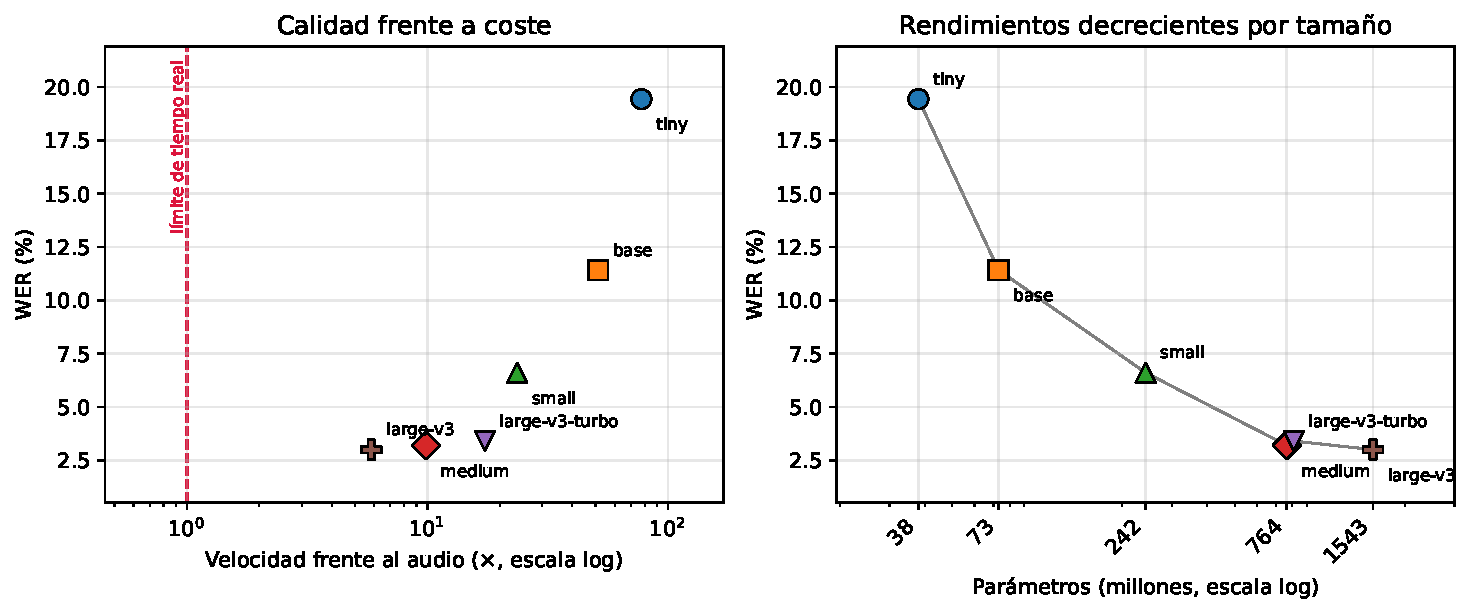
\includegraphics[width=\textwidth]{figuras/baseline_modelos_fleurs_es_fallback.pdf}
\caption{Calidad frente a coste y rendimientos decrecientes por tamaño de modelo. La línea
vertical marca el límite de tiempo real. Generada desde los datos de ejecución.}
\label{fig:modelos}
\end{figure}

% GENERADO AUTOMATICAMENTE por research/eval/report/tabla_corpus.py
% No editar a mano.
\begin{table}[h]
\centering
\small
\begin{tabular}{|l|l|l|r|r|r|r|r|r|r|}
    \hline
    \textbf{Corpus} & \textbf{Variedad} & \textbf{Registro} & \textbf{tiny} & \textbf{base} & \textbf{small} & \textbf{medium} & \textbf{large--v3--turbo} & \textbf{large--v3} & \textbf{$\Delta$ tildes} \\
    \hline
    \texttt{fleurs-es} & Latinoamérica & Leída, enciclopédica & 19.44 & 11.42 & 6.61 & 3.21 & 3.41 & 3.01 & -- \\
    \texttt{tedx-es} & México & Charla espontánea & -- & -- & 12.13 & 10.22 & 11.12 & -- & $-$3.48 \\
    \texttt{teleconciencia-es} & México & Divulgación científica & -- & -- & 23.42 & 18.61 & 22.26 & -- & $-$5.11 \\
    \texttt{mediaspeech-es} & Peninsular & Medios, locución & -- & -- & 15.94 & 14.72 & 15.60 & -- & $-$1.70 \\
    \texttt{voxpopuli-es} & Peninsular & Parlamentario & -- & -- & 12.01 & 10.44 & 11.53 & -- & $-$0.07 \\
    \hline
\end{tabular}
\caption{WER (\%) de los modelos Whisper sin adaptar segun corpus, con normalizacion
basica. La columna $\Delta$ tildes indica cuanto baja el WER de \texttt{medium} al
ignorar la acentuacion: valores altos delatan referencias con tildes omitidas (R11), no
mejor reconocimiento.}
\label{tab:baseline-corpus}
\end{table}


Dos observaciones condicionan el resto del trabajo.

La primera: en material de habla espontánea, aumentar el tamaño del modelo deja de
compensar. Entre \texttt{medium} y \texttt{large-v3-turbo} la diferencia es nula, y entre
\texttt{small} y \texttt{medium} apenas 1,5 puntos sobre el corpus más difícil, frente a
los 3,2 que separan los mismos modelos en voz leída. El margen que queda no está en el
tamaño; ese es precisamente el supuesto que motiva estudiar la adaptación.

La segunda: lo que domina el error no es la variedad dialectal sino el registro. A registro
equivalente, el español peninsular y el mexicano dan cifras casi idénticas: 10,44\% frente
a 10,22\%. Lo que lleva el error del 3\% al 23\% es leer un texto frente a hablar de forma
espontánea.

\subsection{El modelo elegido y por qué no es el más rápido}

La primera lectura recomendaba \texttt{large-v3-turbo}: igualaba a \texttt{medium} en tasa
de error y era el doble de rápido. Esa lectura ignoraba el modo de fallo.

Contabilizando las salidas anómalas, entendidas como transcripciones con menos de un cuarto
de las palabras esperadas, \texttt{turbo} produjo tres sobre 180 fragmentos y
\texttt{medium} ninguna. Y no son truncamientos inocuos: en varios fragmentos el modelo
emitió una frase fluida, gramatical y plausible en el dominio que no guardaba relación con
lo dicho.

Para un sistema de accesibilidad ese criterio pesa más que unas décimas de tasa de error.
Un subtítulo ausente se nota; uno inventado, no: el alumno con discapacidad auditiva no
tiene forma de detectarlo porque se lee perfectamente bien. Se eligió \texttt{medium}.

\section{Comparativa de técnicas de adaptación}

% GENERADO AUTOMATICAMENTE por research/eval/report/tabla_tecnicas.py
% No editar a mano.
\begin{table}[h]
\centering
\small
\begin{tabular}{|l|l|r|r|r|c|r|c|}
    \hline
    \textbf{Técnica} & \textbf{Corpus} & \textbf{WER base} &
    \textbf{WER téc.} & \textbf{$\Delta$ (pp)} & \textbf{IC 95\%} &
    \textbf{$p$} & \textbf{Signif.} \\
    \hline
    Prompting contextual & \texttt{tedx-es} & 10.15 & 9.96 & -0.19 & [-0.61, +0.00] & 1.000 & No \\
    Prompting contextual & \texttt{teleconciencia-es} & 18.79 & 19.14 & +0.35 & [-0.52, +1.42] & 0.012 & No \\
    Prompting contextual & \texttt{voxpopuli-es} & 9.99 & 9.60 & -0.39 & [-1.14, +0.45] & 0.375 & No \\
    Post-corrección con LLM & \texttt{teleconciencia-es} & 19.55 & 22.77 & +3.23 & [+2.66, +3.84] & 0.000 & Sí \\
    Post-corrección con LLM & \texttt{voxpopuli-es} & 12.50 & 12.15 & -0.35 & [-1.69, +1.12] & 1.000 & No \\
    \hline
\end{tabular}
\caption{Efecto de cada técnica de adaptación sobre el WER (\%), con diseño pareado.
$\Delta$ negativo indica mejora. El intervalo de confianza se obtiene por bootstrap
remuestreando clips; $p$ corresponde al test de signos sobre los clips que cambian.}
\label{tab:comparativa-tecnicas}
\end{table}


\subsection{Prompting contextual}

La técnica aporta al decodificador un glosario del dominio como contexto previo. El
glosario se extrae de fragmentos disjuntos de los que se evalúan; construirlo con las
transcripciones de evaluación sería una fuga de información y cualquier mejora medida
sería falsa.

El resultado no es concluyente, y lo interesante es que no lo es de dos maneras
incompatibles: sobre el corpus mexicano el efecto es de $+0{,}35$ puntos y sobre el
peninsular de $-0{,}37$. En ambos casos los dos criterios estadísticos discrepan entre sí.
Un efecto cuyo signo se invierte entre corpus y cuyas pruebas no coinciden no es un efecto
pequeño: es la firma de la ausencia de efecto.

La métrica de terminología matiza esa conclusión. Sobre el corpus grande, el prompting
aumenta la cobertura de términos del glosario en 1,42 puntos mientras reduce su precisión
en 1,04: recupera términos que antes se perdían, y a cambio empieza a introducirlos donde
no los hay. El desglose de errores lo confirma desde el otro lado, con 66 sustituciones
menos pero 43 inserciones y 74 omisiones más. El modelo acierta más veces \emph{qué}
palabra es, y falla más veces \emph{si} la palabra estaba.

\subsection{Post-corrección con un modelo de lenguaje local}

Un modelo de lenguaje corrige la transcripción ya producida. La salida del reconocedor
queda fija, de modo que la única variable es la corrección.

La técnica degrada de forma significativa, y el resultado se replicó sobre dos corpus con
características opuestas: $+3{,}23$ puntos sobre referencias con erratas y $+1{,}18$ sobre
referencias verificadas manualmente. La diferencia de magnitud entre ambos es en sí misma
informativa: buena parte del efecto medido inicialmente era un artefacto de la calidad de
la referencia, y la cifra defendible es la del corpus limpio.

El mecanismo se observa directamente en las transcripciones. El modelo sustituye palabras
por sinónimos más precisos, expande siglas, corrige la gramática del hablante y completa lo
que interpreta como intención:

\begin{quote}
\texttt{cirugía} $\rightarrow$ \texttt{quirófano} \\
\texttt{Instituto de Tecnología de la UNAM} $\rightarrow$ \texttt{Universidad Nacional
Autónoma de México (UNAM)} \\
\texttt{atiendan a como un tipo terapia} $\rightarrow$ \texttt{atiendan cómo un tipo de
terapia}
\end{quote}

Cada una de esas ediciones mejora el texto como pieza escrita y lo empeora como
transcripción; son objetivos en conflicto, y un modelo entrenado para generar lenguaje
natural optimiza el primero.

El caso más ilustrativo es otro: en un fragmento, el corrector sustituyó el nombre de una
persona por el nombre de una enfermedad, quedándose con el tema del programa. El resultado
es fluido, gramatical y completamente falso.

Conviene declarar una limitación de este resultado. La primera versión de las instrucciones
dadas al corrector era puramente prohibitiva, y con ella la técnica quedó inerte: ningún
fragmento modificado a nivel de palabra, y errores evidentes sin corregir. Añadir ejemplos
de qué sí debía corregirse la activó. El experimento mide, por tanto, una implementación
concreta y no la técnica en abstracto.

\subsection{Ajuste fino con LoRA}

Es la única de las tres que modifica los pesos del modelo, y la única que mejora de forma
concluyente: 1,23 puntos de reducción del error, con intervalo de confianza
$[-1{,}75, -0{,}77]$ y ambos criterios de acuerdo. El entrenamiento empleó 1.500 fragmentos
(4,64 horas) durante 15,8 minutos, y produjo un adaptador de 18,9~MB frente a los 3~GB del
modelo completo.

La partición de entrenamiento y la de evaluación provienen de divisiones oficiales
distintas del mismo corpus, de modo que la separación no depende de un reparto propio.

El resultado exige un matiz. La caída del error sobre contenido crítico, de 17,52\% a
6,12\%, procede casi toda de los numerales, y el motivo se ve contando dígitos: la
referencia escribe los números en letra y el modelo base los escribía en cifra. El ajuste
fino aprendió esa convención de transcripción. Es adaptación real, pero de estilo y no de
reconocimiento acústico. Un fragmento lo ilustra: donde la referencia dice
\texttt{uno seiscientos ochenta y seis}, el modelo base escribió \texttt{1 686} y el
ajustado \texttt{cero cero seis}; acertó el formato y falló el número, y ambas métricas lo
premiaron. Descontando los numerales, la mejora sobre contenido crítico es real pero
modesta: de 7,7\% a 6,2\%.

\section{El WER no basta para evaluar accesibilidad}

Cuatro observaciones independientes, obtenidas a lo largo del trabajo, apuntan a la misma
conclusión: la métrica habitual del campo oculta precisamente los fallos que perjudican al
usuario final.

\textbf{Contenido crítico.} Sobre el corpus grande, con una tasa de error de palabra del
18,61\%, que suena aceptable, el sistema pierde o altera el 28\% de las negaciones e
introduce trece que nadie pronunció. Perder una preposición se reconstruye por contexto;
perder un \emph{no} invierte la frase. El WER cuenta ambos errores igual.

\textbf{Alucinaciones fluidas.} Los modelos producen ocasionalmente texto verosímil y falso
en lugar de fallar de forma visible. Al tratarse de salidas gramaticales y coherentes con
el dominio, ni el WER agregado ni el usuario final las detectan.

\textbf{Terminología.} El prompting contextual no mueve el WER pero sí recupera términos
del glosario. Sin una métrica específica, la técnica habría parecido completamente
inocua cuando en realidad tiene un efecto dirigido.

\textbf{Duplicación por solapamiento.} Un defecto de implementación que multiplicaba texto
en las fronteras entre ventanas elevaba el WER por encima del 100\%, pero pasó inadvertido
en las pruebas automáticas y solo se detectó al leer una transcripción real.

De estas observaciones surgieron dos instrumentos complementarios: una métrica de
cobertura y precisión sobre la terminología del dominio, y otra que contabiliza los errores
sobre negaciones, numerales y cuantificadores, es decir, sobre las unidades cuya
alteración cambia el significado y no solo la forma.

\section{Desarrollo de la aplicación}

\subsection{Arquitectura}

El sistema separa estrictamente el núcleo investigador del aplicado: la aplicación depende
de una interfaz de reconocimiento y no del código de los experimentos. Esa frontera permitió
incorporar el adaptador ganador al sistema desplegado sin modificar una sola línea de la
aplicación.

La topología es de un emisor y múltiples receptores. El docente captura desde su equipo;
el alumnado únicamente visualiza. Todo el reconocimiento ocurre una vez en el servidor,
con independencia del número de clientes conectados: un diseño donde cada cliente
transcribiera exigiría una unidad de cálculo por alumno, lo que contradice el objetivo de
que un centro pueda desplegarlo.

El acceso queda restringido a la red local por la propia aplicación, que rechaza cualquier
conexión ajena a un rango privado. Se difunde audio de aula con voces identificables; la
restricción no puede depender de que nadie configure mal un reenvío de puertos.

\subsection{Troceado del audio: latencia frente a calidad}

El subtitulado en vivo no puede esperar a que termine la intervención: hay que trocear. La
pregunta es cuánto cuesta cada segundo de latencia que se ahorra.

Un barrido de tamaños de ventana mostró que trocear cada $N$ segundos degrada de forma
sustancial: con ventanas de tres segundos el error casi se duplica respecto a transcribir
el fragmento completo. El motivo son los cortes arbitrarios, que caen en mitad de palabra
o de sintagma justo donde el modelo necesita contexto.

Esa hipótesis se contrastó cortando en los silencios en lugar de por reloj. Los resultados
aparecen en la tabla~\ref{tab:vad}.

\begin{table}[h]
\centering
\small
\begin{tabular}{|l|r|r|r|}
\hline
\textbf{Estrategia} & \textbf{WER} & \textbf{Duración media} & \textbf{p95} \\
\hline
Ventana fija, tope 3~s & 19,85\% & 2,68~s & 3,00~s \\
Silencios, tope 8~s & \textbf{12,48\%} & 2,93~s & 5,92~s \\
Sin trocear (referencia) & 10,44\% & --- & --- \\
\hline
\end{tabular}
\caption{Segmentación por silencios frente a ventana fija, a latencia media equivalente.}
\label{tab:vad}
\end{table}

A latencia media prácticamente idéntica, segmentar por silencios reduce el error 7,4
puntos y se queda a dos del techo que marca transcribir sin trocear. El mecanismo se ve en
las duraciones: con tope de ocho segundos, la segmentación por pausas produce segmentos de
2,9 segundos de media porque el tope casi nunca se alcanza. El resultado son segmentos
cortos y completos, en lugar de cortos y partidos.

El precio es la previsibilidad: el percentil 95 pasa de 3,00 a 5,92 segundos. La latencia
media mejora, pero el peor caso empeora; en accesibilidad esa distinción importa y ambas
cifras deben reportarse.

Se comprobó además si arrastrar la transcripción anterior como contexto entre ventanas
mejoraba los cortes. No aporta: el efecto es de $+0{,}14$ puntos con ventana fija y
$+0{,}61$ con segmentación por silencios. La explicación encaja con lo anterior: cuando los
cortes caen en pausas, cada segmento ya es una unidad coherente, de modo que el contexto no
añade información que falte pero sí arrastra los errores del segmento previo.

\subsection{Requisito de hardware}

Ejecutar el reconocimiento en unidad de procesamiento gráfico no es una comodidad sino un
requisito: el modelo elegido alcanza 8,1 veces la velocidad del audio en GPU y solo 1,6 en
procesador convencional. Descontado el troceado, esa segunda cifra no llega a tiempo real.

\subsection{Robustez frente al ruido de aula}

Se caracterizó la degradación mediante ruido añadido de dos tipos: blanco, estacionario, y
murmullo sintetizado superponiendo voces del propio corpus. Los resultados aparecen en la
tabla~\ref{tab:ruido}.

\begin{table}[h]
\centering
\small
\begin{tabular}{|l|r|r|}
\hline
\textbf{Relación señal-ruido} & \textbf{Ruido blanco} & \textbf{Murmullo} \\
\hline
Audio limpio & 10,44\% & 10,44\% \\
20~dB & 10,50\% & 11,66\% \\
15~dB & 10,57\% & 11,19\% \\
10~dB & 13,23\% & 12,41\% \\
5~dB & 13,98\% & 14,26\% \\
0~dB & 16,85\% & \textbf{36,02\%} \\
\hline
\end{tabular}
\caption{Degradación frente al ruido según relación señal-ruido y tipo de ruido.}
\label{tab:ruido}
\end{table}

Hasta 15~dB la degradación es despreciable, lo que sitúa un micrófono de solapa corriente
en zona segura y permite formular el requisito de captación en términos concretos. Pero el
fallo no es gradual: entre 5 y 0~dB con murmullo el error se triplica, mientras que el
ruido blanco al mismo nivel apenas lo altera. La diferencia confirma el mecanismo: lo que
arruina el reconocimiento no es la energía del ruido sino que comparta espectro con la voz.
Seis voces de fondo enmascaran lo que un ventilador no, y por eso los supresores de ruido
convencionales, diseñados para ruido estacionario, no resuelven el problema del aula.

\section{Incidentes metodológicos}
\label{sec:incidentes}

Varios de los resultados anteriores estuvieron a punto de ser erróneos. Se documentan
porque comparten una característica que los hace peligrosos: en todos los casos el sistema
seguía funcionando y produciendo cifras verosímiles.

\textbf{La configuración de decodificación como factor de confusión.} Con decodificación
voraz, uno de los modelos truncaba seis de cada cuarenta fragmentos y llegaba a emitir
frases plausibles del dominio en lugar del contenido real; su tasa de error subía de 11,5\%
a 24,2\%. Comparar técnicas sin fijar esta configuración habría medido artefactos de
decodificación en lugar del efecto de la adaptación. Desde entonces, la decodificación
forma parte del nombre de cada fichero de resultados.

\textbf{Sobrescritura del corpus.} Al ampliar un corpus de 40 a 1.200 fragmentos se
sobrescribió su manifiesto; los resultados anteriores seguían apuntando a un fichero cuyo
contenido ya era otro, y nada lo delataba. La corrección fue doble: registrar el resumen
criptográfico del manifiesto en cada resultado, para detectar la discrepancia, y permitir
que varias muestras de la misma fuente convivan, para prevenirla.

\textbf{Un entrenamiento roto que no daba error.} El primer ajuste con LoRA terminó
correctamente, guardó su adaptador y produjo métricas evaluables, con la función de pérdida
estancada en 6,87 y subiendo entre épocas. La causa era que el preparador de lotes
descartaba un identificador de token equivocado, de modo que el decodificador recibía
duplicado el marcador de inicio. Corregido, la pérdida cayó a 0,21. De no haberse
detectado, la evaluación habría mostrado que el ajuste fino destroza el modelo, con
intervalo estrecho y significación respaldando un artefacto.

\textbf{Ajustar sobre referencias defectuosas.} Uno de los corpus disponibles omite las
tildes de forma sistemática. Entrenar sobre él habría enseñado al modelo a no acentuar y,
medido contra esas mismas referencias, la tasa de error \emph{habría mejorado}: se habría
optimizado hacia el error con la métrica dando la razón.

\textbf{Un preprocesado que anula la segmentación.} Al probar la aplicación con micrófono
real, casi todos los segmentos se cerraban por agotar el tope en lugar de por pausa. La
causa no estaba en el algoritmo sino en el control automático de ganancia del navegador:
al callar el hablante sube la ganancia, amplifica el ruido de fondo y la energía nunca
desciende lo suficiente. Es un efecto que ningún experimento sobre audio grabado podía
detectar, porque solo existe cuando hay un micrófono y un navegador de por medio.

Este último incidente ilustra la relación entre los dos núcleos del trabajo mejor que
cualquier argumento: la investigación proporcionó a la aplicación su criterio de diseño,
y la aplicación descubrió una condición sin la cual ese criterio no se cumple.

\chapter{Conclusiones y Trabajo Futuro}
\label{cap:conclusiones}

\section{Conclusiones}

\subsection{Sobre las técnicas de adaptación}

De las tres técnicas evaluadas, solo mejora la que modifica los pesos del modelo. El
ajuste fino con LoRA reduce el error 1,23 puntos con ambos criterios estadísticos de
acuerdo; el prompting contextual no produce efecto detectable, con signo distinto en cada
corpus y pruebas que discrepan entre sí; y la post-corrección con un modelo de lenguaje
local lo empeora de forma significativa y replicada.

La conclusión sobre la post-corrección merece detenerse, porque contradice la intuición
del campo. Un modelo de lenguaje debería poder reparar errores de reconocimiento usando el
contexto, y sin embargo degrada. El mecanismo observado explica por qué: el corrector
optimiza la calidad del texto como pieza escrita, sustituyendo palabras por sinónimos más
precisos y corrigiendo la gramática del hablante, mientras que una transcripción debe
reflejar lo dicho. Son objetivos en conflicto, y el modelo optimiza el que le corresponde
por entrenamiento.

Sobre LoRA cabe un matiz que conviene no omitir: buena parte de su mejora consiste en
aprender la convención de escritura del corpus de ajuste, no en reconocer mejor el audio.
Descontado ese efecto, la ganancia sigue existiendo pero es modesta.

\subsection{Sobre dónde está realmente el margen de mejora}

El resultado más relevante del trabajo no procede de la comparativa de técnicas sino de su
comparación con las decisiones de ingeniería del sistema. Segmentar el audio por silencios
en lugar de por reloj reduce el error 7,4 puntos a igual latencia media; seis veces más que
la mejor de las técnicas de adaptación, y a coste de cómputo prácticamente nulo.

Esto invierte la premisa de la que partía el trabajo. Se asumía que el margen estaba en
adaptar el modelo al dominio educativo; los datos indican que, con los modelos actuales, el
margen está en cómo se le entrega el audio. Un sistema de subtitulado en vivo que trocee
mal desperdicia más calidad de la que cualquier técnica de adaptación puede recuperar.

\subsection{Sobre la evaluación}

La tasa de error de palabra es insuficiente para valorar un sistema de accesibilidad, y el
trabajo aporta cuatro evidencias independientes de ello. La más contundente: con un 18,61\%
de error, cifra que suena aceptable, el sistema pierde o altera el 28\% de las negaciones e
introduce trece que nadie pronunció. Un alumno con discapacidad auditiva lee entonces lo
contrario de lo explicado, sin ninguna señal de que algo falla.

De ahí se derivan dos instrumentos que se proponen como complemento: una métrica de
cobertura y precisión sobre la terminología del dominio, y otra que contabiliza los errores
sobre negaciones, numerales y cuantificadores. Ambas detectan efectos que el WER agregado
no muestra, y en un caso concreto invierten la valoración de una técnica.

\subsection{Sobre la validez de las mediciones}

Cinco incidentes documentados en la sección~\ref{sec:incidentes} comparten una
característica: en todos ellos el sistema seguía funcionando y produciendo cifras
verosímiles. Ninguno se manifestó como un error.

La conclusión práctica es que un procedimiento experimental en este campo necesita
comprobaciones que no forman parte del procedimiento habitual: verificar que la función de
pérdida esté en el rango esperado antes de evaluar un modelo ajustado; auditar a mano una
muestra de las referencias antes de adoptar un corpus; incorporar la configuración de
decodificación a la identidad del resultado; y registrar el contenido exacto del corpus
empleado, no solo su nombre.

\section{Limitaciones}
\label{sec:limitaciones}

\textbf{Ninguno de los corpus es una clase real.} Es la limitación de fondo. Los materiales
empleados se aproximan al registro de una clase magistral, pero ninguno lo es. Las
conclusiones sobre adaptación al dominio educativo son, en rigor, conclusiones sobre
adaptación a los dominios sustitutos disponibles. El corpus objetivo, un repositorio
universitario con transcripciones manuales, requiere una solicitud institucional que quedó
cursada sin resolución dentro del plazo de este trabajo.

\textbf{Los resultados miden implementaciones, no técnicas.} Se hizo evidente con la
post-corrección: una primera versión de las instrucciones dejaba la técnica inerte, y otra
la activaba. Un prompt distinto, un modelo mayor o un ajuste de hiperparámetros podrían
alterar las conclusiones.

\textbf{El detector de actividad de voz es de energía.} Un detector entrenado sería más
robusto frente al ruido de aula, y la práctica del sector indica que la combinación de
ambos reduce sustancialmente las falsas activaciones. La medición realizada justifica
introducirlo, pero no se ha implementado.

\textbf{El ruido se añadió de forma sintética.} Falta la reverberación, que es un factor
independiente y posiblemente más dañino que el ruido aditivo en un aula real.

\textbf{La aplicación no se ha evaluado con usuarios.} Se ha verificado su funcionamiento
técnico y se ha medido su latencia, pero no se ha comprobado si el resultado es útil para
quien debe leerlo.

\textbf{El sistema depende de un único servidor.} La difusión se resuelve en memoria, lo
que ata el despliegue a un proceso. Escalar a varios exigiría una infraestructura
adicional; para un aula no aplica, pero condiciona cualquier extensión a nivel de centro.

\section{Trabajo futuro}

\textbf{Corpus educativo real.} Es la continuación prioritaria: repetir la comparativa
sobre clases grabadas convertiría las conclusiones actuales, obtenidas sobre dominios
sustitutos, en conclusiones sobre el dominio objetivo.

\textbf{Detección de actividad de voz entrenada.} La segmentación resultó ser la palanca
más eficaz del sistema, y actualmente se apoya en el método más simple posible. Mejorarla
es la vía con mayor rendimiento esperable por unidad de esfuerzo.

\textbf{Glosario procedente del material docente.} La extracción automática por frecuencia
produce vocabulario corriente que el modelo ya reconoce. Un glosario elaborado a partir del
temario o las transparencias tendría el contenido que la técnica necesita, y permitiría
reevaluar el prompting en condiciones justas.

\textbf{Métricas de comprensión.} Las métricas propuestas miden la supervivencia de
unidades léxicas concretas. El paso siguiente sería medir si el alumno entiende lo mismo
leyendo la transcripción que escuchando la clase, lo que exige evaluación con personas.

\textbf{Implementaciones optimizadas para inferencia.} Existen variantes del modelo
significativamente más rápidas que la empleada, cuyo soporte para la plataforma de cálculo
utilizada en este trabajo era limitado. Su viabilidad debería reevaluarse, porque el margen
de latencia condiciona directamente la usabilidad en aula.


\bibliographystyle{apacite}
\bibliography{bibliografia}

\appendix
\chapter{Reproducibilidad}
\label{ap:reproducibilidad}

Este apéndice recoge lo necesario para reproducir cualquier cifra de la memoria. No es
documentación de instalación: es la respuesta a la pregunta de si los resultados
presentados pueden volver a obtenerse y con qué grado de fidelidad.

\section{Entorno de ejecución}

Los experimentos se ejecutaron sobre una tarjeta gráfica AMD con la pila de cómputo ROCm,
en un sistema Linux. Esta elección tiene una consecuencia que conviene declarar: parte del
software habitual del campo asume tarjetas de otro fabricante, y algunas implementaciones
optimizadas para inferencia no estaban disponibles. La comparativa se realizó por tanto
sobre la implementación de referencia de la biblioteca \emph{Transformers}
\cite{wolf2020transformers}, más lenta que las alternativas especializadas pero disponible
por igual en ambas plataformas, lo que evita que la elección de hardware se confunda con una
diferencia de resultados.

El intérprete de Python se creó reutilizando los paquetes del sistema de forma deliberada,
porque reinstalar la biblioteca de cálculo dentro del entorno aislado rompe el soporte de
la tarjeta gráfica. Es un detalle menor que causa horas de depuración si se desconoce.

\section{Trazabilidad de los resultados}

El procedimiento actual hace que cada ejecución produzca un fichero de resultados que
registra, junto a las métricas:

\begin{itemize}
  \item El identificador del commit del código que la produjo.
  \item Si el árbol de trabajo tenía cambios sin confirmar en ese momento, lo que indica
        que el commit registrado no basta para reconstruir el estado exacto.
  \item El resumen criptográfico del manifiesto de corpus empleado, junto con su número de
        fragmentos, y el de la submuestra efectiva cuando el experimento evalúa solo una
        parte de él.
  \item La configuración completa: modelo, estrategia de decodificación, semilla,
        parámetros del experimento y versiones de las bibliotecas relevantes.
\end{itemize}

El tercer punto se incorporó tras un incidente. Al ampliar un corpus se sobrescribió su
manifiesto, y los resultados anteriores quedaron apuntando a un fichero cuyo contenido ya
era distinto sin que nada lo advirtiera. El resumen criptográfico permite detectar esa
discrepancia; posteriormente se añadió también la posibilidad de que varias muestras de la
misma fuente coexistan, que la previene.

\subsection*{Hasta dónde llega, en la práctica}

Decir «cada ejecución registra» describe el procedimiento, no el archivo: el mecanismo
nació de aquel incidente, de modo que alcanza en distinto grado a lo ejecutado antes y
después. Conviene dar las cifras, porque presentar la trazabilidad como una propiedad
uniforme sería justamente el tipo de afirmación de la que este trabajo dedica un capítulo a
desconfiar. Sobre los cincuenta y dos ficheros de resultados que sostienen esta memoria:

\begin{itemize}
  \item Todos registran su configuración completa, que es lo que permite repetir la
        ejecución, y todos registran un identificador de commit.
  \item En cuarenta y cuatro ese identificador vale \texttt{sin-git}, porque se produjeron
        antes de que el trabajo estuviera bajo control de versiones. Son los más antiguos,
        y entre ellos está el barrido de línea base.
  \item Once registran el resumen criptográfico del manifiesto, que es la parte que se
        añadió tras el incidente. En los once, recalcularlo hoy devuelve el valor que el
        fichero declara.
  \item Uno solo se produjo con el árbol de trabajo limpio. El resto de los que lo declaran
        tenían cambios sin confirmar, cosa que el propio bloque advierte y que significa
        que el commit registrado no basta para reconstruir el estado exacto.
\end{itemize}

El programa \texttt{tools/auditar\_resultados.py} recorre el archivo entero y falla si algo
no cuadra. Aplica dos comprobaciones, según lo que cada fichero permita.

La directa consiste en \emph{recalcular} el resumen criptográfico del manifiesto y
compararlo con el que el resultado declara. Merece subrayarse por lo que tiene de lección
repetida: guardar el resumen no detecta nada por sí solo, y durante un tiempo nadie lo
recalculó, de modo que la salvaguarda contra el incidente era exactamente la misma clase de
fallo que este trabajo documenta en otros sitios, un dato declarado que ninguna
comprobación consulta. Cuando el experimento evalúa solo una parte del manifiesto se
compara además el resumen de esa submuestra, porque el del fichero completo identifica
material que no se ha medido.

La indirecta cubre a los resultados anteriores al mecanismo, que no llevan resumen: el
número de fragmentos y de palabras de referencia que declara cada fichero tiene que
coincidir con el que produce el manifiesto de hoy. Hoy señala cinco ficheros, y son
precisamente los del incidente: mediciones sobre cuarenta fragmentos de un corpus que
después se amplió a mil doscientos. Ese es el motivo de que la
tabla~\ref{tab:baseline-corpus} marque esa fila, y de que las comparaciones entre modelos
deban hacerse sobre las tablas por corpus.

Dos categorías quedan fuera de la comprobación indirecta sin que eso sea un hueco. Los
barridos de ingeniería vuelven a trocear el audio en ventanas o segmentos, así que no
declaran un recuento de fragmentos con el que contrastar; llevan resumen criptográfico, que
es la comprobación fuerte. Y los experimentos que emplean glosario reservan una fracción de
los fragmentos para extraerlo y evalúan sobre el resto, de modo que su recuento queda por
debajo del manifiesto a propósito: el programa descuenta esa reserva, porque denunciar como
deriva la propia salvaguarda contra la fuga de información habría enterrado los cinco casos
reales bajo cuatro falsos.

Merece una advertencia de uso, porque costó tiempo: el recuento de palabras que guardan los
resultados es el de las referencias \emph{ya normalizadas}, y el normalizador convierte los
signos en espacios, de modo que un corpus puede declarar más palabras de las que tiene en
crudo. Compararlo contra el texto sin normalizar produce discrepancias que no existen.

\subsection*{Qué se versiona y qué no}

Los manifiestos de corpus, los programas y las tablas y figuras generadas están en el
repositorio. No lo están, deliberadamente, tres cosas: el audio, porque su licencia no
permite redistribuirlo; los ficheros de resultados en crudo, porque son la salida de los
programas y no su entrada; y el adaptador entrenado, por tamaño.

La consecuencia hay que decirla sin adornos: \textbf{regenerar cualquier cifra con un solo
comando es cierto sobre una instalación que ya tenga el corpus descargado}, que es el
supuesto en el que se ha trabajado. Un tercero que parta del repositorio necesita antes
obtener el audio de sus fuentes originales mediante los programas de descarga incluidos,
disponer de una tarjeta gráfica, y reentrenar el adaptador para reproducir el resultado del
ajuste fino. Los manifiestos hacen esa reconstrucción posible y verificable, que es su
función; no la hacen inmediata.

\section{Identidad de un resultado}

Los ficheros de resultados se nombran según el modelo, el corpus y la estrategia de
decodificación empleados. Esta última forma parte del nombre porque se comprobó que dos
ejecuciones idénticas salvo por ese parámetro producían tasas de error que diferían en más
de doce puntos. Un resultado identificado únicamente por modelo y corpus habría permitido
comparar cifras no comparables.

La regla general que se derivó: cualquier eje de variación que se introduzca debe
incorporarse al nombre del resultado, no solo a su contenido.

\section{Generación de tablas y figuras}

Ninguna cifra de esta memoria se ha transcrito manualmente. Las tablas y figuras se generan
mediante programas que leen los ficheros de resultados y producen directamente el código
LaTeX o el gráfico correspondiente, que la memoria incorpora por inclusión.

La consecuencia práctica es que regenerar los informes tras una nueva ejecución actualiza
la memoria sin intervención. La consecuencia metodológica es más relevante: una cifra
copiada a mano deja de estar vinculada a la ejecución que la produjo en el momento en que
se copia, y no hay forma de detectar la divergencia posterior.

\section{Verificaciones previas}

Tres comprobaciones se ejecutan antes de dar por válido un resultado, y las tres surgieron
de errores que no producían ningún fallo visible.

\textbf{Verificación de la tarjeta gráfica.} No basta con comprobar que el sistema la
detecta: se verifica que calcula correctamente y que completa un ciclo de entrenamiento con
descenso efectivo de la función de pérdida.

\textbf{Verificación del entrenamiento.} Antes de evaluar un modelo ajustado se comprueba
que la función de pérdida se encuentra en el rango esperado y que desciende entre épocas.
Un ajuste con las etiquetas mal alineadas termina sin errores, guarda su resultado y
produce métricas evaluables; solo el valor absoluto de la pérdida lo delata.

\textbf{Verificación del procesamiento por lotes.} Agrupar fragmentos acelera
sustancialmente los barridos, pero solo es admisible si no altera las transcripciones. Se
comprueba comparándolas con las obtenidas de una en una. Una optimización que cambia los
resultados no es una optimización: es un factor de confusión.

\section{Estructura del repositorio}

El trabajo separa estrictamente el material de investigación del de la aplicación; ambos
no comparten código y se comunican mediante una interfaz documentada. Cada experimento
reside en su propia carpeta, con el programa que lo ejecuta, una descripción de su
hipótesis y su diseño, y sus resultados.

Los manifiestos de corpus se versionan; el audio no. Un manifiesto contiene las rutas, las
transcripciones de referencia, las duraciones y los metadatos disponibles, de modo que el
material puede reconstruirse desde su fuente original sin almacenar los ficheros de sonido.

\chapter{Registro de riesgos}
\label{ap:riesgos}

Este apéndice recoge el registro de riesgos que guió la ejecución del trabajo. Se incluye
por dos motivos. El primero es que varias decisiones de diseño de los capítulos anteriores
no se entienden sin él: no se eligieron por ser las mejores en abstracto, sino por ser las
que sobrevivían a un riesgo concreto. El segundo es que seis de los dieciséis riesgos
\emph{no} estaban previstos: se detectaron midiendo, no planificando, y esa es en sí misma
una observación sobre cómo se planifica un trabajo de esta naturaleza.

\section{Riesgos previstos en la planificación inicial}

Los diez de la tabla~\ref{tab:riesgos-previstos} se identificaron antes de empezar a
medir. Dos de ellos se materializaron, y que estuvieran previstos es lo que evitó que
descarrilaran el trabajo.

\begin{table}[h]
\centering
\footnotesize
\setlength{\tabcolsep}{4pt}
\begin{tabular}{|c|p{5.1cm}|p{5.6cm}|c|}
\hline
\textbf{Id} & \textbf{Riesgo} & \textbf{Mitigación aplicada} & \textbf{Estado} \\
\hline
R1 & No existe corpus educativo en español con transcripción de referencia fiable y de
     acceso abierto & Dos planes aplicados: corpus públicos con el desajuste de dominio
     medido y declarado, y subtítulos existentes verificados a mano. El tercero, la
     solicitud institucional del corpus objetivo, queda redactado y dirigido pero su
     tramitación excede el plazo & Materializado \\
\hline
R2 & Entrenar sobre tarjeta gráfica AMD puede resultar inviable & Verificar en la primera
     fase que la tarjeta \emph{entrena}, con un ciclo mínimo, antes de comprometer la
     técnica que lo necesita & Mitigado \\
\hline
R3 & Datos insuficientes para el ajuste fino & Última en el orden de ejecución y segunda en
     el de recorte; no comprometerla hasta resolver R1 y R2 & No materializado \\
\hline
R4 & Latencia insuficiente para operar en directo & Instrumentar la medida desde el primer
     prototipo y reportar la latencia real aunque no cumpla & Mitigado \\
\hline
R5 & El doble núcleo duplica el trabajo & Tratar la aplicación como vehículo de
     demostración y banco de pruebas, no como contribución con validación propia &
     Materializado \\
\hline
R6 & La comparativa no arroja diferencias concluyentes & Protocolo congelado de antemano
     para que un resultado negativo siga siendo defendible; reportar variabilidad y no solo
     medias & Materializado \\
\hline
R7 & Redacción tardía & Escribir desde la primera fase, en borradores parciales & Mitigado \\
\hline
R8 & Resultados no reproducibles & Una configuración por experimento, semillas fijadas,
     procedencia en cada salida, tablas generadas y no copiadas & Mitigado \\
\hline
R9 & Tratamiento de datos personales & No grabar material propio; el corpus empleado tiene
     licencia de investigación. La restricción de red la impone la aplicación & Mitigado \\
\hline
R10 & Disponibilidad personal & Planificación en fases relativas y puntos de recorte
      explícitos & Mitigado \\
\hline
\end{tabular}
\caption{Riesgos identificados durante la planificación.}
\label{tab:riesgos-previstos}
\end{table}

R1 se materializó en su forma más costosa: el corpus objetivo no se obtuvo, y el trabajo se
ejecutó sobre sustitutos. R6 también, y de ahí que dos de las tres técnicas evaluadas no
produzcan efecto concluyente. Que ambos estuvieran previstos es lo que permitió que su
materialización no descarrilara el trabajo: el criterio de significación y la política de
marcar como no concluyente lo que no alcanza potencia estaban fijados antes de saber qué
iban a dar los datos.

\section{Riesgos detectados midiendo}

Los seis siguientes no aparecían en la planificación. Se documentan aparte porque comparten
un rasgo, visible en la tabla~\ref{tab:riesgos-emergentes}: ninguno se manifestó como un
problema, sino como un resultado creíble.

\begin{table}[h]
\centering
\footnotesize
\setlength{\tabcolsep}{4pt}
\begin{tabular}{|c|p{5.1cm}|p{5.6cm}|c|}
\hline
\textbf{Id} & \textbf{Riesgo} & \textbf{Mitigación aplicada} & \textbf{Estado} \\
\hline
R11 & La calidad de la transcripción de referencia varía entre corpus y se confunde con
      rendimiento del modelo & Auditoría manual de una muestra antes de adoptar cualquier
      corpus; reportar el error con y sin normalización de tildes como cota superior e
      inferior & Mitigado \\
\hline
R12 & Efecto suelo: sobre voz leída el modelo sin adaptar ya acierta casi todo y no queda
      margen donde las técnicas puedan demostrar nada & Trasladar la comparativa al material
      de habla espontánea, donde el error base deja margen & Mitigado \\
\hline
R13 & Desajuste de variedad dialectal entre corpus y destino & Medido: a registro
      equivalente la diferencia entre variedades es de dos décimas, frente a los veinte
      puntos que separa el registro. Queda descartado como factor & Descartado \\
\hline
R14 & La configuración de decodificación es un factor de confusión que mueve el error hasta
      trece puntos & Congelarla e incorporarla a la identidad de cada resultado & Mitigado \\
\hline
R15 & Decisiones de alcance bloqueadas a la espera de validación externa & Tomar decisiones
      provisionales documentadas y marcadas como revisables, con cola viva de preguntas
      pendientes; avanzar mientras tanto en lo que no depende de terceros & Materializado \\
\hline
R16 & El modelo base envejece durante el desarrollo y la elección deja de estar justificada
      & Medirlo en lugar de argumentarlo: contraste con una arquitectura distinta sobre 800
      fragmentos, y catálogo de modelos auditados que se revisa igual que el de corpus &
      Mitigado \\
\hline
\end{tabular}
\caption{Riesgos detectados durante la ejecución, ausentes de la planificación inicial.}
\label{tab:riesgos-emergentes}
\end{table}

R14 y R16 merecen un comentario conjunto, porque ilustran los dos extremos del mismo
problema. R14 era invisible desde dentro: dos ejecuciones del mismo modelo sobre el mismo
corpus daban cifras incomparables y nada lo delataba. R16 era invisible desde fuera: los
resultados seguían siendo correctos, y lo que envejecía era su premisa. Ninguno de los dos
habría aparecido en una revisión del código o de los resultados; el primero exigió comparar
ejecuciones que no debían diferir, y el segundo mirar fuera de la familia de modelos
elegida.

R15 condicionó el método de trabajo más que ningún otro. La norma adoptada ante cualquier
decisión de alcance que no pudiera cerrarse en el momento fue la misma: elegir una opción
razonable por defecto, dejar constancia escrita del motivo en un registro de decisiones y
marcarla como revisable, en lugar de detener el trabajo. El coste de esa política es que
varias decisiones quedan documentadas y argumentadas pero pendientes de validación; el
beneficio es que ninguna de ellas bloqueó el avance del resto.

\chapter{Despliegue y uso del sistema}
\label{ap:despliegue}

El capítulo~\ref{cap:desarrollo} explica \emph{por qué} el despliegue tiene la forma que
tiene. Este apéndice explica \emph{cómo} se ejecuta, paso a paso, y está escrito para quien
tenga que ponerlo en marcha en un centro sin haber participado en el desarrollo: el
responsable informático el primer día, y el docente cada mañana.

\section{Qué hace falta antes de empezar}

El sistema se despliega en \textbf{un solo equipo del centro}, que actúa de servidor y hace
todo el trabajo. Los dispositivos del alumnado no necesitan absolutamente nada salvo un
navegador y estar en la misma red: no instalan, no calculan y no conceden permisos. Esa
asimetría es deliberada y se justifica en la sección~\ref{sec:arquitectura-app}; para el
despliegue lo que implica es que solo hay un equipo del que preocuparse.

Los requisitos de ese equipo no son una lista de recomendaciones: cada uno procede de una
medición del capítulo~\ref{cap:desarrollo} y puede comprobarse antes de dar una clase con el
sistema. Se presentan en dos tablas porque responden a dos preguntas distintas: la
tabla~\ref{tab:requisitos-despliegue} dice \emph{qué equipo hace falta}, que es una decisión
de compra, y la tabla~\ref{tab:requisitos-entorno} \emph{qué hay que preparar} en el que ya
se tenga.

\begin{table}[!ht]
\centering
\footnotesize
\setlength{\tabcolsep}{4pt}
\begin{tabular}{|p{2.5cm}|p{3.3cm}|p{6.2cm}|}
\hline
\textbf{Elemento} & \textbf{Requisito} & \textbf{De dónde sale} \\
\hline
Tarjeta gráfica &
    Dedicada, con al menos \textbf{4~GB} de memoria propia. No hace falta gama alta. &
    Medido: el modelo ocupa 1,60~GB de memoria de vídeo en el peor caso
    (tabla~\ref{tab:huella}). El resto es margen para el escritorio del propio equipo y la
    fragmentación de memoria. Sin tarjeta dedicada el sistema arranca, pero no sostiene el
    ritmo del audio en directo (sección~\ref{sec:hardware}). \\
\hline
Memoria del sistema &
    \textbf{8~GB}. &
    El proceso de reconocimiento ocupa 2,76~GB residentes; la aplicación y el sistema
    operativo caben holgadamente en el resto. \\
\hline
Procesador &
    Cuatro núcleos o más. Cualquiera de los últimos años sirve. &
    No calcula el modelo: despacha el trabajo a la tarjeta gráfica. Conviene saber que
    \textbf{un núcleo queda ocupado al 100\% de forma permanente} mientras el servicio está
    vivo, incluso en reposo: es espera activa del entorno de ejecución de la GPU, no trabajo
    real, y no indica ningún problema. \\
\hline
Almacenamiento &
    Depende de la vía: \textbf{5~GB} nativa, \textbf{100~GB} en contenedores sobre AMD. &
    El modelo son 2,85~GB en ambos casos. La diferencia no la causa el sistema sino la
    imagen base de la plataforma de AMD, y se detalla más abajo porque es lo bastante grande
    como para condicionar la elección de equipo. \\
\hline
\end{tabular}
\caption{Requisitos de hardware del equipo servidor, con la medición que respalda cada uno.}
\label{tab:requisitos-despliegue}
\end{table}

\begin{table}[!ht]
\centering
\footnotesize
\setlength{\tabcolsep}{4pt}
\begin{tabular}{|p{2.5cm}|p{3.3cm}|p{6.2cm}|}
\hline
\textbf{Elemento} & \textbf{Requisito} & \textbf{Observación} \\
\hline
Sistema operativo &
    Linux permite el despliegue en contenedores; en macOS con Apple Silicon hay que
    ejecutar de forma nativa. &
    No es indiferente: en macOS los contenedores no alcanzan la GPU. Conviene leer la
    sección~\ref{sec:contenedores} \emph{antes} de elegir procedimiento. \\
\hline
Acceso a la GPU &
    Con AMD, pertenecer a los grupos \texttt{video} y \texttt{render}. Con NVIDIA, el
    conjunto de herramientas de contenedores del fabricante. &
    Es el fallo de arranque más frecuente. Se comprueba con
    \texttt{getent group video render}, cuyos identificadores numéricos deben coincidir con
    los del descriptor de contenedores. \\
\hline
Micrófono &
    De solapa o diadema, próximo a la boca del docente. No vale el micrófono integrado del
    equipo ni uno ambiental. &
    Medido: el sistema tolera ruido hasta 15~dB de relación señal-ruido, y por debajo se
    degrada de golpe en lugar de gradualmente (sección~\ref{sec:ruido}). La proximidad del
    micrófono es lo que mantiene ese margen cuando el aula se anima. \\
\hline
Red &
    Red local del centro, con el equipo servidor y los dispositivos del alumnado en el
    mismo rango. &
    La aplicación rechaza toda conexión que no provenga de un rango privado. No es
    configurable: es un requisito legal del sistema
    (sección~\ref{sec:requisitos-legales}). Si hiciera falta acceso desde fuera, la vía es
    una red privada virtual hasta el centro. \\
\hline
Navegador &
    Cualquiera moderno, tanto en el equipo del docente como en los del alumnado. &
    La emisión debe abrirse en el propio equipo servidor, por una restricción de los
    navegadores que se explica en el paso 4. \\
\hline
\end{tabular}
\caption{Requisitos de entorno y periféricos.}
\label{tab:requisitos-entorno}
\end{table}

Conviene señalar lo que \emph{no} aparece en ninguna de las dos, porque suele darse por supuesto: no
hace falta conexión a internet durante la clase, ni cuenta en ningún servicio, ni licencia de
software. La única descarga es la del modelo, y ocurre una sola vez en el primer arranque.
Esto es consecuencia directa de que el reconocimiento se ejecute en el centro y no en la nube
(sección~\ref{sec:requisitos-legales}).

\subsection*{De dónde salen esas cifras}

Los tres requisitos de memoria y almacenamiento proceden de una medición directa del
servicio en ejecución, no del tamaño nominal del modelo, que es lo que suele citarse y
además induce a error. La tabla~\ref{tab:huella} recoge el detalle.

% GENERADO AUTOMATICAMENTE por research/eval/report/tabla_huella.py
% No editar a mano.
\begin{table}[H]
\centering
\small
\begin{tabular}{|l|r|r|r|}
    \hline
    \textbf{Modelo} & \textbf{Disco (GB)} & \textbf{VRAM pico (GB)} &
    \textbf{RAM del proceso (GB)} \\
    \hline
    \texttt{whisper-small} & 0.90 & 0.56 & 2.57 \\
    \texttt{whisper-medium} & 2.85 & 1.60 & 2.76 \\
    \texttt{whisper-medium + LoRA} & 2.85 & 1.63 & 2.78 \\
    \hline
\end{tabular}
\caption{Huella de recursos del servicio de reconocimiento, medida sobre
AMD Radeon RX 9070 XT con precisión \texttt{float16} y una ventana completa de 30~s de audio, que
es el caso peor. El pico de VRAM mayor observado es 1.63~GB, de donde sale el
requisito de 4~GB de la tabla~\ref{tab:requisitos-despliegue}: el margen cubre el
gestor de ventanas del propio equipo y la fragmentación de memoria.}
\label{tab:huella}
\end{table}


Dos lecturas de esa tabla importan para decidir la compra. La primera es que el requisito de
memoria de vídeo es \textbf{mucho menor de lo que sugiere el tamaño del modelo en disco}:
2,85~GB ocupados en almacenamiento se traducen en 1,60~GB de memoria de vídeo, porque los
pesos se cargan en precisión reducida. Una tarjeta de 4~GB, que hoy es la gama de entrada,
sobra. Lo que el sistema necesita no es una tarjeta grande sino, simplemente, una tarjeta.

La segunda es que existe una salida si el equipamiento disponible se queda corto: el modelo
inmediatamente menor baja el pico a 0,56~GB y el almacenamiento a 0,90~GB. Cuesta calidad,
entre uno y dos puntos de tasa de error según el material
(tabla~\ref{tab:baseline-modelos-tedx-es}), pero es una degradación conocida y medida, no una
sorpresa. La diferencia entre ambos modelos se estrecha además precisamente en habla
espontánea, que es el registro del aula.

Incorporar el modelo adaptado no cambia el cuadro: el adaptador añade 19~MB en disco y
30~MB de memoria de vídeo, porque no sustituye al modelo sino que le agrega unas matrices
pequeñas. Es la ventaja práctica de la técnica que ganó la comparativa, y la razón de que
pueda distribuirse por separado.

\subsection*{El almacenamiento, que es la sorpresa desagradable}

Las cifras anteriores se refieren al modelo. El despliegue completo en contenedores sobre
AMD ocupa mucho más, y conviene decirlo con claridad porque es el requisito que más se
subestima:

\begin{table}[H]
\centering
\footnotesize
\begin{tabular}{|l|r|}
\hline
\textbf{Componente} & \textbf{Disco} \\
\hline
Imagen del reconocimiento (AMD) & 83,5~GB \\
\hline
Caché de núcleos de cálculo compilados & 11,6~GB \\
\hline
Caché del modelo & 3,1~GB \\
\hline
Imagen de la aplicación & 0,35~GB \\
\hline
\textbf{Total aproximado} & \textbf{$\sim$100~GB} \\
\hline
\end{tabular}
\caption{Ocupación en disco del despliegue en contenedores sobre AMD, medida con
\texttt{docker system df -v} en el equipo de desarrollo.}
\label{tab:disco}
\end{table}

Lo llamativo es de dónde viene: \textbf{no es el modelo}, que son 2,85~GB, sino la imagen
base de la plataforma de cálculo de AMD. Inspeccionarla por dentro explica el motivo, y el
motivo es que el contenedor transporta código para tarjetas que el equipo no tiene.

Esa plataforma compila por anticipado los núcleos de cálculo para cada arquitectura de
tarjeta, y la imagen empleada los incluye \emph{todos}: su etiqueta declara literalmente
\texttt{device-all}. Medido dentro de ella, una sola de sus bibliotecas de álgebra contiene
núcleos para \textbf{veinticuatro arquitecturas distintas}, desde las de centro de datos
hasta tres generaciones de tarjetas de consumo; de sus 792~MB, los que corresponden a la
tarjeta empleada en este trabajo son \textbf{10~MB}. Otro componente aparece como trece
bibliotecas separadas, una por arquitectura, que suman 4,4~GB y de las que se usa una.

A ello se añaden dos circunstancias más. La imagen incluye el kit de \emph{desarrollo} de la
plataforma, 15~GB de compiladores y cabeceras que no hacen falta para ejecutar inferencia
pese a que la imagen se anuncia como de ejecución. Y los 11,6~GB de núcleos compilados en el
primer arranque se generan porque, para la generación de tarjeta concreta empleada, esa
plataforma no distribuye binarios precompilados y hay que producirlos en destino.

Conviene precisar el grado de confianza de las cifras. Las de la tabla proceden de
\texttt{docker system df -v}, que es lo que el sistema informa; el contenido real del sistema
de ficheros de la imagen, medido desde dentro, son 34~GiB. La diferencia se debe a cómo el
motor de contenedores contabiliza capas almacenadas y desplegadas, y no se ha podido acotar
con precisión por requerir privilegios de administrador sobre su directorio de datos. Para
planificar un despliegue conviene por tanto tomar la cifra alta, que es la conservadora.

Tres consecuencias prácticas. La primera, que un equipo con un disco pequeño, que es lo
habitual en un portátil de centro, puede quedarse sin espacio por esta vía y no por el
modelo. La segunda, que la ejecución nativa ocupa alrededor de 5~GB y evita el problema por
completo, lo que la convierte en una alternativa razonable y no en un apaño. La tercera, que
esto es reducible: partir de una imagen base restringida a la familia de tarjeta del equipo,
en lugar de a todas, eliminaría por construcción la mayor parte de lo que se transporta. No
se ha hecho, de modo que no se aporta la cifra resultante; queda como la mejora pendiente
más rentable del despliegue.

Hay una última observación que afecta menos al espacio y más a la reproducibilidad, y por eso
conviene dejarla escrita: la imagen base empleada es una compilación \textbf{nocturna} y no
una versión estable, según declaran sus propios parámetros de construcción. Para el
desarrollo es aceptable, porque era la vía de tener soporte de una tarjeta muy reciente; para
un despliegue en un centro no lo es, porque la referencia se mueve bajo los pies y dos
construcciones separadas en el tiempo no producen el mismo sistema. Fijar una versión estable
concreta es requisito previo a cualquier distribución, y es coherente con el criterio que
gobierna el resto del trabajo: un resultado que no se puede reconstruir no es un resultado.

Del perfil de NVIDIA no se da cifra porque no se ha medido: no se dispuso de una tarjeta de
ese fabricante. Cabe esperar que sea sustancialmente menor, porque su imagen base es de
ejecución y no de desarrollo, pero es una expectativa y no un dato.

\section{Cómo se distribuye el sistema}
\label{sec:contenedores}

\subsection*{Qué es un contenedor, y por qué se usa aquí}

El sistema se entrega \textbf{contenerizado}. Un contenedor es un paquete que incluye el
programa junto con todas sus dependencias, es decir el intérprete, las bibliotecas y sus
versiones exactas, de modo que se ejecuta igual en cualquier equipo que tenga el motor de
contenedores instalado, sin instalar nada más en el sistema anfitrión. Docker es la implementación
empleada aquí, y es la habitual.

La razón de recurrir a ello no es seguir una moda de despliegue: es que el entorno de este
sistema es especialmente incómodo de montar a mano. Requiere una versión concreta de la
biblioteca de cálculo, compilada contra la plataforma del fabricante de la tarjeta gráfica,
más el entorno de ejecución de la aplicación. Reproducir eso en el equipo de un centro sería
una tarde de trabajo para alguien con conocimientos, y una fuente permanente de averías al
actualizar el sistema operativo. Con contenedores, el centro instala Docker y ejecuta un
comando.

El sistema se reparte en \textbf{dos contenedores} y no en uno, porque tienen necesidades
distintas: el del reconocimiento necesita acceso a la tarjeta gráfica y pesa varios
gigabytes; el de la aplicación web no necesita tarjeta y es pequeño. Separarlos permite
además sustituir el modelo sin tocar la aplicación, que es la frontera descrita en la
sección~\ref{sec:integracion}.

\subsection*{Sobre qué sistemas operativos se puede ejecutar}

\begin{table}[H]
\centering
\footnotesize
\setlength{\tabcolsep}{4pt}
\begin{tabular}{|p{3.1cm}|c|c|p{5.6cm}|}
\hline
\textbf{Sistema} & \textbf{Vía} & \textbf{Acelerador} & \textbf{Estado} \\
\hline
Linux, tarjeta AMD & Contenedores & ROCm &
    \texttt{make docker-amd}. Es la plataforma de desarrollo del trabajo. \\
\hline
Linux, tarjeta NVIDIA & Contenedores & CUDA &
    \texttt{make docker-nvidia}. Requiere el conjunto de herramientas de contenedores del
    fabricante. \\
\hline
macOS, Apple Silicon & \textbf{Nativa} & MPS &
    \texttt{make demo}. En contenedor no alcanza la GPU; se explica más abajo. \\
\hline
Windows, como cliente & \multicolumn{3}{p{8.4cm}|}{\textbf{Funciona sin nada especial.} Es
    solo un navegador. Es además el caso más frecuente: los dispositivos del alumnado.} \\
\hline
Windows, como servidor & \multicolumn{3}{p{8.4cm}|}{No probado. Existe una vía a través del
    subsistema Linux de Windows, pero el descriptor de contenedores requiere cambios; se
    detalla más abajo.} \\
\hline
Sin tarjeta gráfica & \multicolumn{3}{p{8.4cm}|}{Arranca y transcribe, pero no sostiene el
    directo. Sirve para verificar la instalación y la red del aula, no para dar clase.} \\
\hline
\end{tabular}
\caption{Sistemas operativos sobre los que puede ejecutarse el servidor.}
\label{tab:vias}
\end{table}

\subsection*{De dónde salen las imágenes}

Conviene ser preciso en esto, porque determina lo que un centro tiene que hacer y lo que
todavía no puede hacer.

\textbf{Las imágenes de este sistema no están publicadas en ningún registro público.} No
existe, por tanto, una orden \texttt{docker pull} que las descargue: se construyen en el
propio equipo a partir del repositorio del proyecto, y eso es lo que hace la opción
\texttt{-{}-build} de los comandos de la tabla~\ref{tab:vias}. El proceso, la primera vez,
consiste en descargar las imágenes base públicas de las que se parte, instalar sobre ellas
las dependencias declaradas y copiar el código del proyecto.

Las imágenes base sí proceden de registros públicos, y son las que recoge la
tabla~\ref{tab:imagenes-base}:

\begin{table}[H]
\centering
\footnotesize
\begin{tabular}{|l|l|}
\hline
\textbf{Componente} & \textbf{Imagen base} \\
\hline
Reconocimiento, AMD & \texttt{rocm/pytorch} \\
\hline
Reconocimiento, NVIDIA & \texttt{pytorch/pytorch:2.5.1-cuda12.4-cudnn9-runtime} \\
\hline
Aplicación, compilación & \texttt{mcr.microsoft.com/dotnet/sdk:10.0} \\
\hline
Aplicación, ejecución & \texttt{mcr.microsoft.com/dotnet/aspnet:10.0} \\
\hline
\end{tabular}
\caption{Imágenes base de las que parten los contenedores del sistema.}
\label{tab:imagenes-base}
\end{table}

La versión concreta de la imagen base del reconocimiento se fija desde fuera y no dentro del
fichero de construcción, a propósito: cada combinación de tarjeta y controlador exige una
distinta, y codificarla obligaría a editar el fichero en cada despliegue.

\textbf{Qué implica que no estén publicadas.} Hoy, el centro necesita el repositorio del
proyecto y una máquina capaz de construir, lo que incluye descargar las dependencias de
compilación de la aplicación. Publicar las imágenes en un registro, por ejemplo el del propio
alojamiento del código, reduciría el despliegue a descargar el descriptor y ejecutar
\texttt{docker compose up}, sin repositorio ni construcción, y haría el primer arranque
mucho más rápido y mucho menos sensible al equipo. Es una mejora de distribución evidente y
queda como tarea pendiente, no como decisión: no se ha hecho porque el trabajo no ha llegado
a la fase de distribuir el sistema a terceros.

\subsection*{El caso de Windows}

Merece tratamiento propio por una razón práctica: es, con diferencia, el sistema más
extendido en los centros educativos españoles, de modo que despacharlo en una línea sería
ignorar el escenario más probable. Conviene separar dos papeles que se confunden con
facilidad.

\textbf{Como cliente no hay nada que hacer.} Los equipos del alumnado, y cualquier pantalla
del aula que solo muestre subtítulos, funcionan con Windows exactamente igual que con
cualquier otro sistema: abren una dirección en el navegador. Este es el caso más frecuente
en la práctica, y conviene decirlo explícitamente porque la advertencia siguiente puede
leerse mal.

\textbf{Como servidor no se ha probado, pero la vía existe.} El sistema no se ha desplegado
sobre Windows en este trabajo, y por tanto no se afirma que funcione. Sí puede describirse
con precisión qué haría falta, porque el obstáculo está localizado.

El camino sería el subsistema Linux de Windows, que hoy permite acceso a la tarjeta gráfica
desde dentro. Tanto la plataforma de NVIDIA \cite{microsoft2024cudawsl} como la de AMD
\cite{amd2025rocmwsl} exponen la tarjeta a través de un dispositivo propio del subsistema,
\texttt{/dev/dxg}, en lugar de los dispositivos que se usan en un Linux nativo. Y ahí está
justamente el problema: \textbf{el perfil de AMD de este proyecto pasa al contenedor
\texttt{/dev/kfd} y \texttt{/dev/dri}, que bajo el subsistema no existen}. Ese perfil
requeriría por tanto modificarse. El de NVIDIA está mejor situado, porque no enumera
dispositivos a mano sino que delega en el conjunto de herramientas del fabricante, que es
precisamente el que se encarga de exponer el dispositivo correcto dentro del contenedor.

Hay un segundo obstáculo, menor pero real: los contenedores comparten la red del anfitrión,
decisión tomada por un problema concreto de la distribución de desarrollo
(sección~\ref{sec:contenedores}). Ese modo se comporta de forma distinta en el entorno de
Docker para Windows, así que habría que volver a publicar puertos, que es lo que se hace
normalmente.

Queda una tercera vía que conviene no perder de vista, porque puede ser la más simple:
\textbf{ejecutar sin contenedores}. Los dos componentes del sistema son de por sí
multiplataforma: la biblioteca de cálculo del servicio de reconocimiento tiene versión para
Windows con tarjetas NVIDIA, y el entorno de ejecución de la aplicación es de Microsoft y
nativo allí. Lo que no es multiplataforma es la automatización del proyecto, que asume un
intérprete de órdenes de tipo Unix; habría que ejecutar los comandos a mano. Tampoco se ha
probado.

En resumen, y para que un centro sepa a qué atenerse: sobre Windows con tarjeta NVIDIA el
despliegue es plausible y probablemente cercano, sobre Windows con tarjeta AMD exige
modificar el descriptor, y en ambos casos habría que verificarlo antes de comprometerse.
Queda recogido como tarea pendiente en lugar de como afirmación.

\subsection*{El caso de Apple Silicon}

Merece explicación aparte porque es contraintuitivo y porque un centro con equipamiento
Apple lo encontrará de inmediato. Afecta a \textbf{toda la gama con chips de la serie M},
tanto portátiles como equipos de sobremesa, porque lo que lo provoca es la arquitectura del
procesador y no el formato del equipo.

Conviene señalarlo porque los equipos de sobremesa de esa gama son, de hecho, candidatos
razonables al papel de servidor de aula: son silenciosos, consumen poco y están pensados
para permanecer encendidos, que es exactamente lo que este sistema necesita. Un centro que
ya disponga de uno tiene una opción sensata, siempre que lo despliegue por la vía correcta.

Y la vía correcta no es la que parecería. La aplicación funciona sin cambios en esa
arquitectura, dentro o fuera de contenedor; el problema está en el servicio de
reconocimiento.

Ejecutado de forma nativa, el servicio detecta el acelerador integrado en el chip y lo
emplea, con una particularidad que el código resuelve solo: fuerza precisión simple, porque
Metal no implementa la precisión reducida para todas las operaciones del modelo y con ella
la inferencia falla o devuelve silencio.

Ejecutado en contenedor, en cambio, \textbf{queda en procesador y no hay forma de evitarlo}.
La causa no es del sistema desarrollado: en macOS los contenedores corren dentro de una
máquina virtual Linux que no expone el acelerador de Apple. Y quedarse en procesador
significa 1,6 veces la velocidad del audio (sección~\ref{sec:hardware}), insuficiente para
directo. De ahí que en estos equipos la vía correcta sea la nativa, aunque sea la menos
cómoda.

Queda una cosa por declarar, porque afecta a cuánta confianza merece esta recomendación:
\textbf{el rendimiento de ese acelerador no se ha medido en este trabajo}. Se ha verificado
que el servicio lo detecta y transcribe correctamente, pero el barrido de dispositivos
comparó únicamente tarjeta gráfica dedicada y procesador (sección~\ref{sec:hardware}).
Además, dentro de la propia gama el rendimiento varía mucho: no es comparable el chip de
entrada de un portátil con las variantes de gama alta de un sobremesa, que multiplican el
número de núcleos gráficos. Un centro que vaya a desplegar sobre este equipamiento debería
medir el factor de tiempo real en su equipo concreto, con el mismo procedimiento del
experimento, antes de comprometerse.

\subsection*{Estado de verificación de cada vía}

Por el mismo motivo se declara aquí, y no en una nota al pie, qué está probado y qué no:

\begin{itemize}
  \item \textbf{Vía nativa sobre Linux con tarjeta AMD:} es la empleada durante todo el
        desarrollo y la que produjo las mediciones de esta memoria. Probada.
  \item \textbf{Vía en contenedores sobre Linux con tarjeta AMD:} \textbf{construida y
        ejecutada}. Los dos contenedores arrancan, superan su comprobación de salud y se
        mantienen en servicio; las cifras de ocupación en disco de la
        tabla~\ref{tab:disco} proceden de ese despliegue. Lo que no se ha hecho es una
        sesión de aula completa a través de ellos.
  \item \textbf{Vía en contenedores sobre Linux con tarjeta NVIDIA:} sin probar, por no
        disponer de una tarjeta de ese fabricante. El descriptor está escrito y difiere del
        anterior solo en la imagen base y en el mecanismo de acceso a la tarjeta.
  \item \textbf{Vía nativa sobre Apple Silicon:} el servicio detecta el acelerador y
        transcribe. Sin medición de rendimiento.
  \item \textbf{Windows, en cualquier variante:} sin probar como servidor. Como cliente
        funciona igual que cualquier otro sistema.
\end{itemize}

Este inventario es deliberado, y su nivel de detalle también. El
capítulo~\ref{cap:desarrollo} documenta varios casos en los que algo funcionaba en
apariencia y producía resultados falsos; dar por verificada una vía de despliegue que nadie
ha ejecutado sería exactamente el mismo error, y darla por no verificada cuando sí se ha
ejecutado tampoco ayuda a quien tenga que desplegarla.

\section{Puesta en marcha}

\subsection*{Paso 1: obtener el proyecto}

Basta con el repositorio; no hay que descargar el modelo a mano, porque el contenedor lo
hace en el primer arranque y lo conserva.

\subsection*{Paso 2: configurar la clave del puesto docente}

Se define en un fichero \texttt{.env} junto al descriptor de los contenedores:

\begin{quote}\ttfamily
CLAVE\_DOCENTE=la-clave-que-elija-el-centro
\end{quote}

\textbf{Este paso no es opcional, y el descriptor de contenedores lo impone.} Sin clave, la
vista de emisión queda abierta y cualquier alumno conectado a la red podría tomarla y
emitir por el aula. Durante un tiempo la variable tenía el valor vacío por defecto, de modo
que seguir estos pasos sin definirla levantaba el sistema desprotegido sin ninguna
advertencia; ahora el arranque se detiene y explica qué falta. La interfaz sigue avisando
además cuando la aplicación corre sin clave, que es el modo de desarrollo.

En el mismo fichero conviene fijar la política de reinicio:

\begin{quote}\ttfamily
REINICIO=unless-stopped
\end{quote}

Con ella, los contenedores vuelven a levantarse solos cuando arranca el equipo, que es lo
que se quiere de un servidor de aula: tras un corte de luz o un reinicio nocturno, el
sistema está disponible sin que nadie tenga que entrar a arrancarlo. El valor por defecto es
el contrario, \texttt{no}, porque en un equipo de desarrollo unos contenedores que resucitan
en cada encendido son una molestia, y el del reconocimiento además mantiene ocupado un
núcleo y varios gigabytes de memoria mientras vive.

Se emplea \texttt{unless-stopped} y no \texttt{always} por una diferencia que importa en un
centro: si alguien detiene el sistema a propósito, debe seguir detenido hasta que se decida
arrancarlo, y no reaparecer en el siguiente encendido.

\subsection*{Paso 3: levantar el sistema}

Un único comando, elegido según la tabla~\ref{tab:vias}:

\begin{quote}\ttfamily
make docker-amd \qquad\qquad\rmfamily(Linux, tarjetas AMD, plataforma ROCm)\\
\ttfamily make docker-nvidia \qquad\rmfamily(Linux, tarjetas NVIDIA, plataforma CUDA)\\
\ttfamily make demo \qquad\qquad\quad\rmfamily(macOS con Apple Silicon, ejecución nativa)
\end{quote}

Entre las dos primeras la diferencia es únicamente la imagen base del servicio de
reconocimiento; el código es idéntico, porque la biblioteca de cálculo expone la misma
interfaz sobre las dos plataformas. La tercera no usa contenedores por el motivo explicado
en la sección~\ref{sec:contenedores}, y requiere tener preparado el entorno de Python y
el de la aplicación en el propio equipo.

\textbf{El primer arranque es lento y eso es normal.} Hay que descargar la imagen base, que
en el caso de AMD son más de ochenta gigabytes (tabla~\ref{tab:disco}), descargar el modelo
y compilar los núcleos de cálculo de la tarjeta. Todo ello queda guardado en volúmenes, de
modo que los arranques siguientes son inmediatos. Conviene por tanto hacer el primer
arranque con un día de margen sobre la primera clase, y con una conexión que aguante esa
descarga.

\subsection*{Paso 4: comprobar que funciona}

El comando anterior imprime al arrancar las dos direcciones del sistema, recogidas en la
tabla~\ref{tab:direcciones}. Son distintas y no son intercambiables:

\begin{table}[H]
\centering
\footnotesize
\begin{tabular}{|l|l|p{6.2cm}|}
\hline
\textbf{Quién} & \textbf{Dirección} & \textbf{Observación} \\
\hline
Docente & \texttt{http://localhost:5203/broadcast} &
    Debe abrirse \textbf{en el propio equipo servidor}. \\
\hline
Alumnado & \texttt{http://<ip-del-equipo>:5203/view} &
    Desde cualquier dispositivo de la misma red. \\
\hline
\end{tabular}
\caption{Direcciones de acceso al sistema.}
\label{tab:direcciones}
\end{table}

La restricción de la primera fila tiene una causa concreta y conviene entenderla antes de
intentar sortearla: los navegadores solo conceden acceso al micrófono en conexiones seguras
o en la máquina local. Como el sistema opera dentro de la red del centro y sin certificado,
\textbf{la emisión tiene que hacerse desde el equipo servidor}. Si se quisiera emitir desde
otro equipo del aula habría que servir la aplicación por HTTPS con un certificado
reconocido por los dispositivos del centro, lo que es perfectamente posible pero excede lo
que este trabajo despliega.

\subsection*{Paso 5: dar clase}

En la vista del docente: introducir la clave, pegar en el recuadro del glosario los términos
de la sesión, uno por línea, y pulsar el botón de comenzar. Los subtítulos aparecen a la vez
en la pantalla del docente y en la de todo el alumnado conectado.

El glosario conviene tomarlo del temario o de las transparencias de la sesión. No hace falta
que sea exhaustivo: sirve para que los términos propios de la asignatura se resalten
visualmente en el subtítulo.

\subsection*{Paso 6: detener el sistema}

\begin{quote}\ttfamily
make docker-parar
\end{quote}

Detiene los contenedores sin borrar el modelo descargado ni las cachés, de modo que el
arranque siguiente vuelva a ser inmediato.

\section{Incorporar el modelo adaptado}

El resultado del ajuste fino se activa añadiendo una línea al mismo fichero \texttt{.env}:

\begin{quote}\ttfamily
ADAPTADOR=/adaptador
\end{quote}

No hay que reconstruir nada ni modificar la aplicación: el servicio de reconocimiento aplica
el adaptador sobre el modelo base al cargarlo. Dejar la variable vacía sirve el modelo sin
adaptar. Es la comprobación práctica de la frontera descrita en la
sección~\ref{sec:integracion}.

\section{Qué hacer si algo no funciona}

Los tres fallos que se han observado en la práctica tienen la misma característica que los
incidentes del capítulo~\ref{cap:desarrollo}: el sistema no se cae, simplemente funciona
peor sin decirlo.

\textbf{Los subtítulos tardan mucho y llegan en bloques largos.} Mirar el contador de la
vista del docente que separa los cortes cerrados \emph{por pausa} de los cerrados \emph{por
agotar el tope}. Si dominan los segundos, el detector de silencios no está encontrando las
pausas. La causa habitual no está en el sistema sino en el navegador: el control automático
de ganancia amplifica el ruido de fondo cuando el hablante calla, y la energía nunca baja lo
suficiente. La aplicación lo desactiva al capturar; si aun así ocurre, revisar que no haya
un procesado de audio activo en el sistema operativo o en el propio micrófono.

\textbf{Aparecen frases que nadie ha dicho.} El sistema filtra los dos patrones
reconocibles, las muletillas de subtítulos de vídeo y los bucles de repetición, pero no
puede filtrar una alucinación verosímil (sección~\ref{sec:filtro}). Si son frecuentes, casi
siempre indica que al micrófono le llega poca voz y mucho fondo: acercarlo al docente antes
que tocar ninguna configuración.

\textbf{La calidad cae de golpe a mitad de clase.} La degradación frente al ruido no es
gradual: el sistema pasa de funcionar bien a fallar en un margen de cinco decibelios
(sección~\ref{sec:ruido}). Si el aula se ha animado, el remedio es el micrófono de
proximidad, no un ajuste del software.

\textbf{El contenedor de reconocimiento no arranca con tarjeta AMD.} Casi siempre son los
identificadores de los grupos \texttt{video} y \texttt{render}, que varían entre equipos y
están fijados numéricamente en el descriptor. Se consultan con
\texttt{getent group video render} y se ajustan.

\section{Arranque sin contenedores}

Los dos atajos que se emplearon durante el desarrollo sirven también para desplegar, y son
la vía obligada en macOS:

\begin{quote}\ttfamily
make app \qquad\rmfamily arranca solo la aplicación, con un motor de reconocimiento
simulado\\
\ttfamily make demo \qquad\rmfamily arranca el servicio de reconocimiento real y la
aplicación, y limpia al salir\\
\ttfamily make demo-lora \quad\rmfamily igual, pero sirviendo el modelo adaptado
\end{quote}

El primero merece atención porque resuelve un problema práctico de despliegue: permite
comprobar que la red del aula, los dispositivos del alumnado y las direcciones de acceso
funcionan \emph{antes} de que entre en juego el reconocimiento. Si los subtítulos simulados
llegan a los móviles de la clase y los reales no, el problema está en el servicio de
reconocimiento; si no llegan ni los simulados, está en la red. Separar esas dos causas
ahorra la mayor parte del tiempo de diagnóstico.


\end{document}
